\documentclass[]{article}
\usepackage{lmodern}
\usepackage{amssymb,amsmath}
\usepackage{ifxetex,ifluatex}
\usepackage{fixltx2e} % provides \textsubscript
\ifnum 0\ifxetex 1\fi\ifluatex 1\fi=0 % if pdftex
  \usepackage[T1]{fontenc}
  \usepackage[utf8]{inputenc}
\else % if luatex or xelatex
  \ifxetex
    \usepackage{mathspec}
  \else
    \usepackage{fontspec}
  \fi
  \defaultfontfeatures{Ligatures=TeX,Scale=MatchLowercase}
  \newcommand{\euro}{€}
\fi
% use upquote if available, for straight quotes in verbatim environments
\IfFileExists{upquote.sty}{\usepackage{upquote}}{}
% use microtype if available
\IfFileExists{microtype.sty}{%
\usepackage{microtype}
\UseMicrotypeSet[protrusion]{basicmath} % disable protrusion for tt fonts
}{}
\usepackage[margin=1in]{geometry}
\usepackage{hyperref}
\PassOptionsToPackage{usenames,dvipsnames}{color} % color is loaded by hyperref
\hypersetup{unicode=true,
            pdftitle={Creating plots in R using ggplot2 - part 7: histograms},
            pdfauthor={Jodie Burchell; Mauricio Vargas Sepúlveda},
            pdfborder={0 0 0},
            breaklinks=true}
\urlstyle{same}  % don't use monospace font for urls
\usepackage{color}
\usepackage{fancyvrb}
\newcommand{\VerbBar}{|}
\newcommand{\VERB}{\Verb[commandchars=\\\{\}]}
\DefineVerbatimEnvironment{Highlighting}{Verbatim}{commandchars=\\\{\}}
% Add ',fontsize=\small' for more characters per line
\usepackage{framed}
\definecolor{shadecolor}{RGB}{248,248,248}
\newenvironment{Shaded}{\begin{snugshade}}{\end{snugshade}}
\newcommand{\KeywordTok}[1]{\textcolor[rgb]{0.13,0.29,0.53}{\textbf{{#1}}}}
\newcommand{\DataTypeTok}[1]{\textcolor[rgb]{0.13,0.29,0.53}{{#1}}}
\newcommand{\DecValTok}[1]{\textcolor[rgb]{0.00,0.00,0.81}{{#1}}}
\newcommand{\BaseNTok}[1]{\textcolor[rgb]{0.00,0.00,0.81}{{#1}}}
\newcommand{\FloatTok}[1]{\textcolor[rgb]{0.00,0.00,0.81}{{#1}}}
\newcommand{\ConstantTok}[1]{\textcolor[rgb]{0.00,0.00,0.00}{{#1}}}
\newcommand{\CharTok}[1]{\textcolor[rgb]{0.31,0.60,0.02}{{#1}}}
\newcommand{\SpecialCharTok}[1]{\textcolor[rgb]{0.00,0.00,0.00}{{#1}}}
\newcommand{\StringTok}[1]{\textcolor[rgb]{0.31,0.60,0.02}{{#1}}}
\newcommand{\VerbatimStringTok}[1]{\textcolor[rgb]{0.31,0.60,0.02}{{#1}}}
\newcommand{\SpecialStringTok}[1]{\textcolor[rgb]{0.31,0.60,0.02}{{#1}}}
\newcommand{\ImportTok}[1]{{#1}}
\newcommand{\CommentTok}[1]{\textcolor[rgb]{0.56,0.35,0.01}{\textit{{#1}}}}
\newcommand{\DocumentationTok}[1]{\textcolor[rgb]{0.56,0.35,0.01}{\textbf{\textit{{#1}}}}}
\newcommand{\AnnotationTok}[1]{\textcolor[rgb]{0.56,0.35,0.01}{\textbf{\textit{{#1}}}}}
\newcommand{\CommentVarTok}[1]{\textcolor[rgb]{0.56,0.35,0.01}{\textbf{\textit{{#1}}}}}
\newcommand{\OtherTok}[1]{\textcolor[rgb]{0.56,0.35,0.01}{{#1}}}
\newcommand{\FunctionTok}[1]{\textcolor[rgb]{0.00,0.00,0.00}{{#1}}}
\newcommand{\VariableTok}[1]{\textcolor[rgb]{0.00,0.00,0.00}{{#1}}}
\newcommand{\ControlFlowTok}[1]{\textcolor[rgb]{0.13,0.29,0.53}{\textbf{{#1}}}}
\newcommand{\OperatorTok}[1]{\textcolor[rgb]{0.81,0.36,0.00}{\textbf{{#1}}}}
\newcommand{\BuiltInTok}[1]{{#1}}
\newcommand{\ExtensionTok}[1]{{#1}}
\newcommand{\PreprocessorTok}[1]{\textcolor[rgb]{0.56,0.35,0.01}{\textit{{#1}}}}
\newcommand{\AttributeTok}[1]{\textcolor[rgb]{0.77,0.63,0.00}{{#1}}}
\newcommand{\RegionMarkerTok}[1]{{#1}}
\newcommand{\InformationTok}[1]{\textcolor[rgb]{0.56,0.35,0.01}{\textbf{\textit{{#1}}}}}
\newcommand{\WarningTok}[1]{\textcolor[rgb]{0.56,0.35,0.01}{\textbf{\textit{{#1}}}}}
\newcommand{\AlertTok}[1]{\textcolor[rgb]{0.94,0.16,0.16}{{#1}}}
\newcommand{\ErrorTok}[1]{\textcolor[rgb]{0.64,0.00,0.00}{\textbf{{#1}}}}
\newcommand{\NormalTok}[1]{{#1}}
\usepackage{graphicx,grffile}
\makeatletter
\def\maxwidth{\ifdim\Gin@nat@width>\linewidth\linewidth\else\Gin@nat@width\fi}
\def\maxheight{\ifdim\Gin@nat@height>\textheight\textheight\else\Gin@nat@height\fi}
\makeatother
% Scale images if necessary, so that they will not overflow the page
% margins by default, and it is still possible to overwrite the defaults
% using explicit options in \includegraphics[width, height, ...]{}
\setkeys{Gin}{width=\maxwidth,height=\maxheight,keepaspectratio}
\setlength{\parindent}{0pt}
\setlength{\parskip}{6pt plus 2pt minus 1pt}
\setlength{\emergencystretch}{3em}  % prevent overfull lines
\providecommand{\tightlist}{%
  \setlength{\itemsep}{0pt}\setlength{\parskip}{0pt}}
\setcounter{secnumdepth}{0}

%%% Use protect on footnotes to avoid problems with footnotes in titles
\let\rmarkdownfootnote\footnote%
\def\footnote{\protect\rmarkdownfootnote}

%%% Change title format to be more compact
\usepackage{titling}

% Create subtitle command for use in maketitle
\newcommand{\subtitle}[1]{
  \posttitle{
    \begin{center}\large#1\end{center}
    }
}

\setlength{\droptitle}{-2em}
  \title{Creating plots in R using ggplot2 - part 7: histograms}
  \pretitle{\vspace{\droptitle}\centering\huge}
  \posttitle{\par}
  \author{Jodie Burchell \\ Mauricio Vargas Sepúlveda}
  \preauthor{\centering\large\emph}
  \postauthor{\par}
  \predate{\centering\large\emph}
  \postdate{\par}
  \date{2016-05-13}



% Redefines (sub)paragraphs to behave more like sections
\ifx\paragraph\undefined\else
\let\oldparagraph\paragraph
\renewcommand{\paragraph}[1]{\oldparagraph{#1}\mbox{}}
\fi
\ifx\subparagraph\undefined\else
\let\oldsubparagraph\subparagraph
\renewcommand{\subparagraph}[1]{\oldsubparagraph{#1}\mbox{}}
\fi

\begin{document}
\maketitle

{
\setcounter{tocdepth}{2}
\tableofcontents
}
This is the seventh tutorial in a series on using \texttt{ggplot2} I am
creating with \href{http://t-redactyl.github.io/}{Jodie Burchell}. In
this tutorial we will demonstrate some of the many options the
\texttt{ggplot2} package has for creating and customising histograms. We
will use R's
\href{https://stat.ethz.ch/R-manual/R-devel/library/datasets/html/airquality.html}{airquality
dataset} in the \texttt{datasets} package.

In this tutorial, we will work towards creating the histogram below. We
will take you from a basic histogram and explain all the customisations
we add to the code step-by-step.

The first thing to do is load in the data and the libraries, as below:

\begin{center}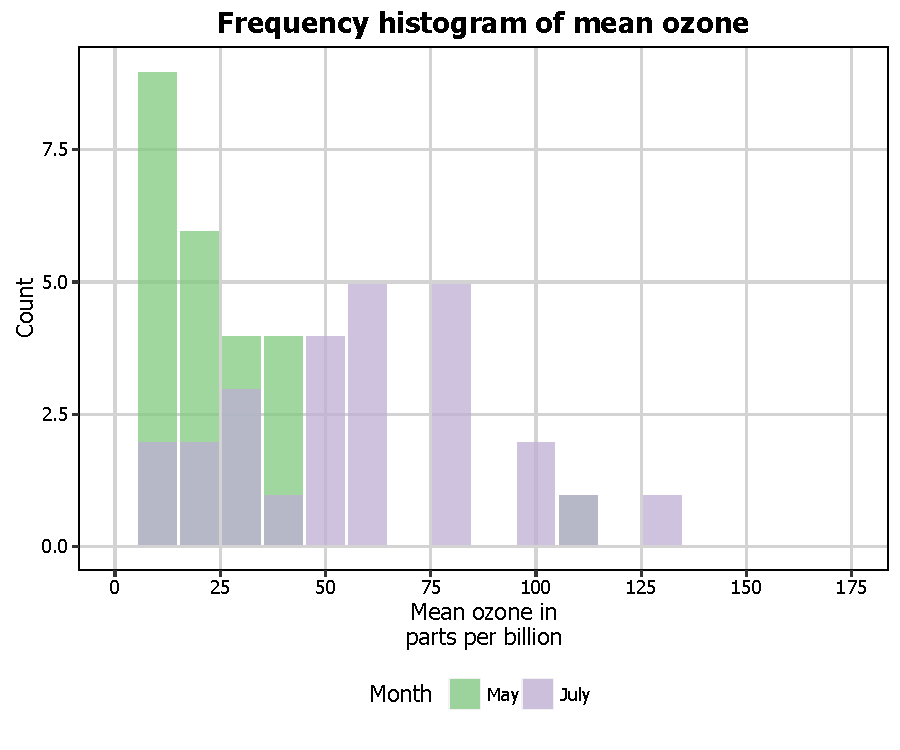
\includegraphics{7_Histograms_pdf/histogram_final-1} \end{center}

The first thing to do is load in the data and the libraries, as below:

\begin{Shaded}
\begin{Highlighting}[]
\KeywordTok{library}\NormalTok{(datasets)}
\KeywordTok{library}\NormalTok{(ggplot2)}
\KeywordTok{library}\NormalTok{(ggthemes)}
\KeywordTok{library}\NormalTok{(extrafont)}
\KeywordTok{library}\NormalTok{(grid)}
\KeywordTok{library}\NormalTok{(RColorBrewer)}

\KeywordTok{data}\NormalTok{(airquality)}
\end{Highlighting}
\end{Shaded}

\section{Basic histogram}\label{basic-histogram}

In order to initialise a plot we tell ggplot that \texttt{airquality} is
our data, and specify that our x axis plots the \texttt{Ozone} variable.
We then instruct ggplot to render this as a histogram by adding the
\texttt{geom\_histogram()} option.

\begin{Shaded}
\begin{Highlighting}[]
\NormalTok{p7 <-}\StringTok{ }\KeywordTok{ggplot}\NormalTok{(airquality, }\KeywordTok{aes}\NormalTok{(}\DataTypeTok{x =} \NormalTok{Ozone)) +}\StringTok{ }\KeywordTok{geom_histogram}\NormalTok{()}
\NormalTok{p7}
\end{Highlighting}
\end{Shaded}

\begin{center}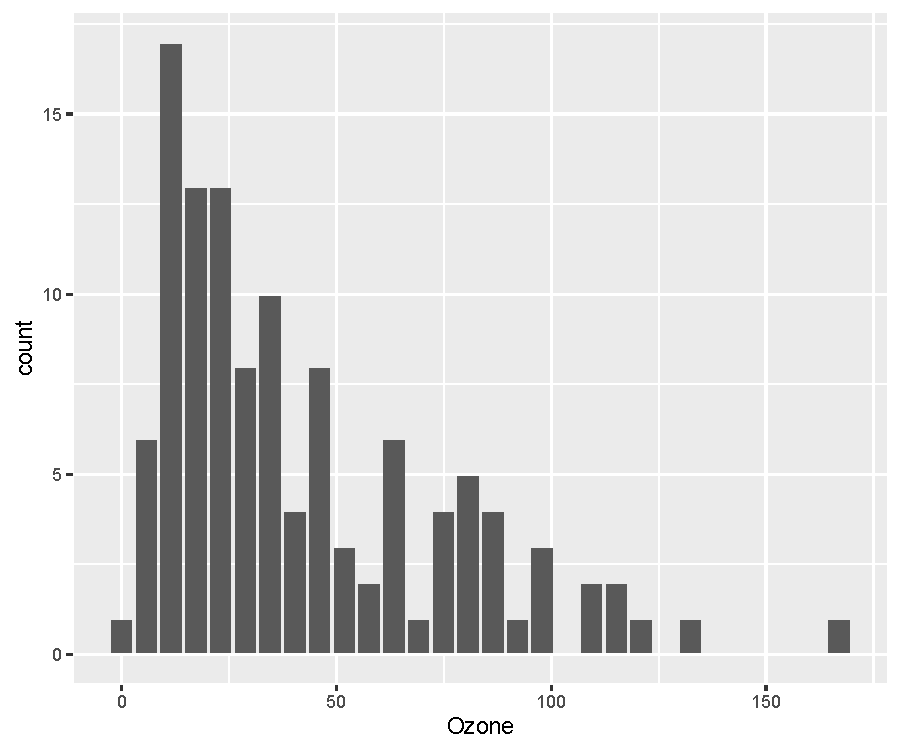
\includegraphics{7_Histograms_pdf/histogram_1-1} \end{center}

\section{Adding a normal density
curve}\label{adding-a-normal-density-curve}

We can overlay a normal density function curve on top of our histogram
to see how closely (or not) it fits a normal distribution. In this case,
we can see it deviates from a normal distribution, showing marked
positive skew. In order to overlay the function curve, we add the option
\texttt{stat\_function(fun\ =\ dnorm)}, and specify the shape using the
\texttt{mean\ =\ mean(airquality\$Ozone)} and
\texttt{sd\ =\ sd(airquality\$Ozone)} arguments. If you have missing
data like we did, make sure you pass the \texttt{na.rm\ =\ TRUE}
argument to the mean and sd parameters. Finally, you can change the
colour using the \texttt{colour\ =\ "red"} argument. We will discuss how
to customise colours further below.

One further change we must make to display the normal curve correctly is
adding \texttt{aes(y\ =\ ..density..)} to the \texttt{geom\_histogram}
option. Note that the normal density curve will not work if you are
using the frequency rather than the density, which we are changing in
our next step.

\begin{Shaded}
\begin{Highlighting}[]
\NormalTok{p7 <-}\StringTok{ }\KeywordTok{ggplot}\NormalTok{(airquality, }\KeywordTok{aes}\NormalTok{(}\DataTypeTok{x =} \NormalTok{Ozone)) +}\StringTok{ }
\StringTok{  }\KeywordTok{geom_histogram}\NormalTok{(}\KeywordTok{aes}\NormalTok{(}\DataTypeTok{y =} \NormalTok{..density..)) +}
\StringTok{  }\KeywordTok{stat_function}\NormalTok{(}\DataTypeTok{fun =} \NormalTok{dnorm, }\DataTypeTok{colour =} \StringTok{"red"}\NormalTok{, }
    \DataTypeTok{args =} \KeywordTok{list}\NormalTok{(}\DataTypeTok{mean =} \KeywordTok{mean}\NormalTok{(airquality$Ozone, }\DataTypeTok{na.rm =} \OtherTok{TRUE}\NormalTok{), }
    \DataTypeTok{sd =} \KeywordTok{sd}\NormalTok{(airquality$Ozone, }\DataTypeTok{na.rm =} \OtherTok{TRUE}\NormalTok{)))}
\NormalTok{p7}
\end{Highlighting}
\end{Shaded}

\begin{center}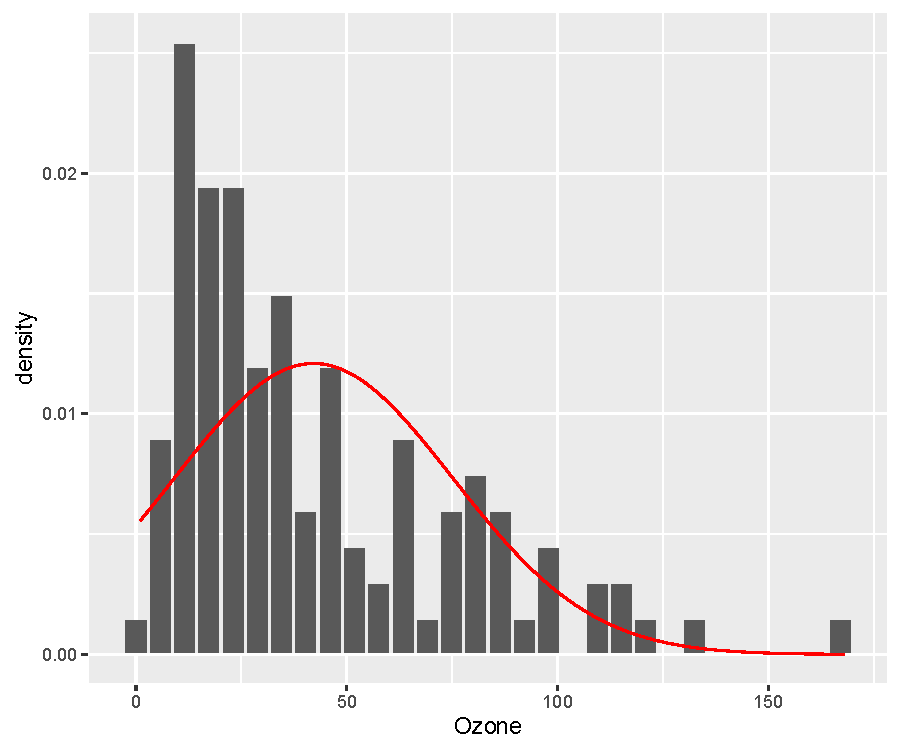
\includegraphics{7_Histograms_pdf/histogram_2-1} \end{center}

\section{Changing from density to
frequency}\label{changing-from-density-to-frequency}

Let's go back to the basic plot and lose the function curve. To change
the y-axis from density to frequency, we add the
\texttt{aes(y\ =\ ..count..)} option to \texttt{geom\_histogram}.

\begin{Shaded}
\begin{Highlighting}[]
\NormalTok{p7 <-}\StringTok{ }\KeywordTok{ggplot}\NormalTok{(airquality, }\KeywordTok{aes}\NormalTok{(}\DataTypeTok{x =} \NormalTok{Ozone)) +}\StringTok{ }
\StringTok{  }\KeywordTok{geom_histogram}\NormalTok{(}\KeywordTok{aes}\NormalTok{(}\DataTypeTok{y =} \NormalTok{..count..))}
\NormalTok{p7}
\end{Highlighting}
\end{Shaded}

\begin{center}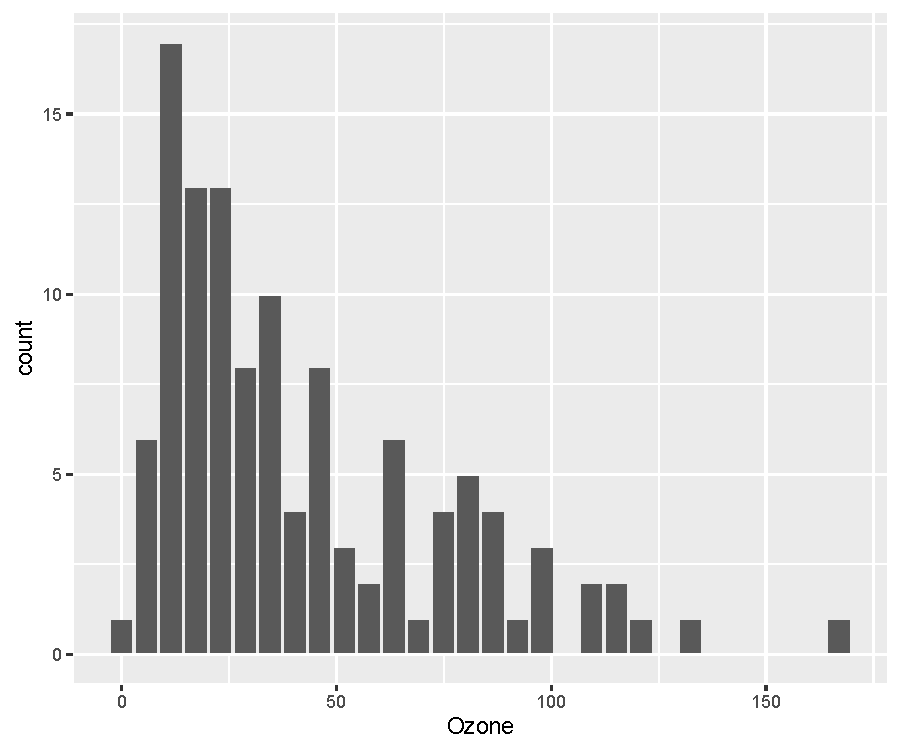
\includegraphics{7_Histograms_pdf/histogram_3-1} \end{center}

\section{Adjusting binwidth}\label{adjusting-binwidth}

To change the binwidth, we add a \texttt{binwidth} argument to
\texttt{geom\_histogram}. In this case, we will make binwidth 5 units of
the \texttt{Ozone} variable.

\begin{Shaded}
\begin{Highlighting}[]
\NormalTok{p7 <-}\StringTok{ }\KeywordTok{ggplot}\NormalTok{(airquality, }\KeywordTok{aes}\NormalTok{(}\DataTypeTok{x =} \NormalTok{Ozone)) +}\StringTok{ }
\StringTok{  }\KeywordTok{geom_histogram}\NormalTok{(}\KeywordTok{aes}\NormalTok{(}\DataTypeTok{y =} \NormalTok{..count..), }\DataTypeTok{binwidth =} \DecValTok{5}\NormalTok{)}
\NormalTok{p7}
\end{Highlighting}
\end{Shaded}

\begin{center}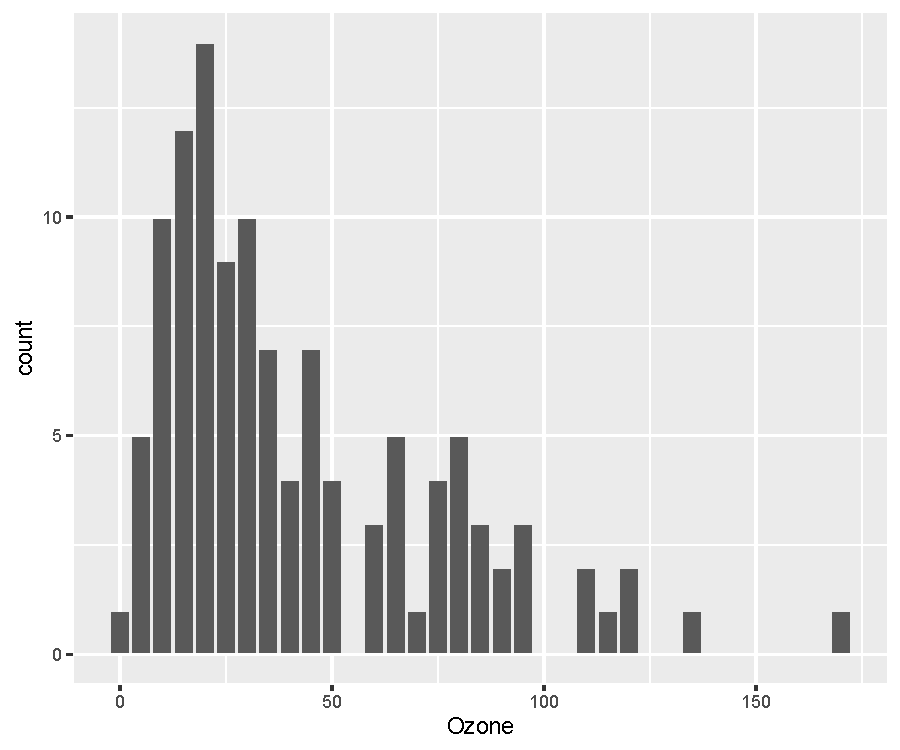
\includegraphics{7_Histograms_pdf/histogram_4-1} \end{center}

\section{Customising axis labels}\label{customising-axis-labels}

\subsection{Single line labels}\label{single-line-labels}

In order to change the axis labels, we have a couple of options. In this
case, we have used the \texttt{scale\_x\_continuous} and
\texttt{scale\_y\_continuous} options, as these have further
customisation options for the axes we will use below. In each, we add
the desired name to the \texttt{name} argument as a string.

\begin{Shaded}
\begin{Highlighting}[]
\NormalTok{p7 <-}\StringTok{ }\KeywordTok{ggplot}\NormalTok{(airquality, }\KeywordTok{aes}\NormalTok{(}\DataTypeTok{x =} \NormalTok{Ozone)) +}\StringTok{ }
\StringTok{  }\KeywordTok{geom_histogram}\NormalTok{(}\KeywordTok{aes}\NormalTok{(}\DataTypeTok{y =} \NormalTok{..count..), }\DataTypeTok{binwidth =} \DecValTok{5}\NormalTok{) +}
\StringTok{  }\KeywordTok{scale_x_continuous}\NormalTok{(}\DataTypeTok{name =} \StringTok{"Mean ozone in parts per billion"}\NormalTok{) +}
\StringTok{  }\KeywordTok{scale_y_continuous}\NormalTok{(}\DataTypeTok{name =} \StringTok{"Count"}\NormalTok{)}
\NormalTok{p7}
\end{Highlighting}
\end{Shaded}

\begin{center}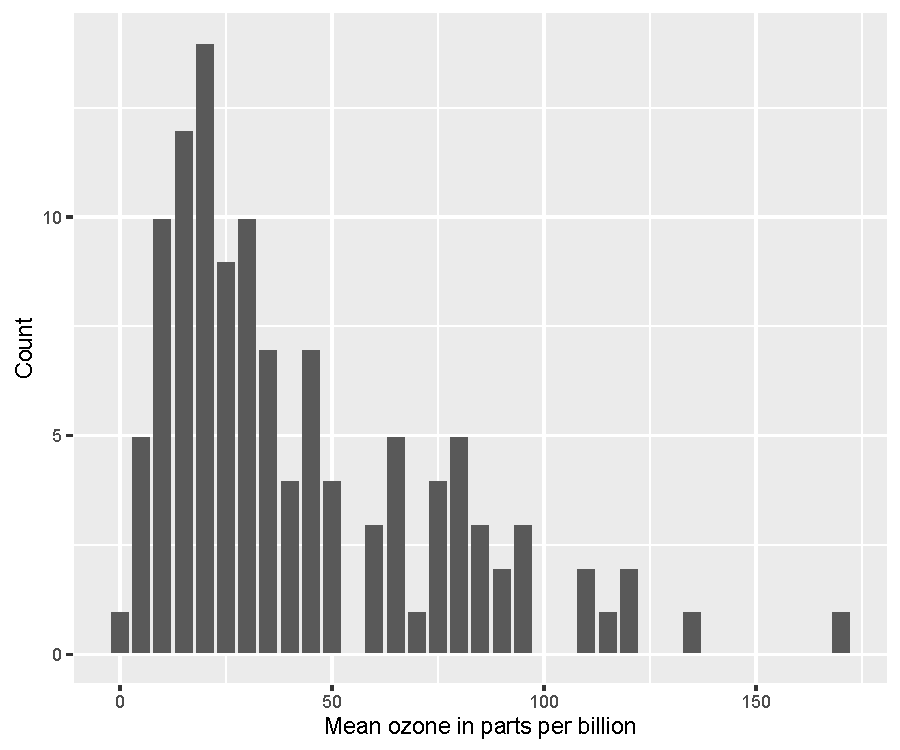
\includegraphics{7_Histograms_pdf/histogram_5-1} \end{center}

\subsection{Multiline labels}\label{multiline-labels}

ggplot also allows for the use of multiline names (in both axes and
titles). Here, we've changed the x-axis label so that it goes over two
lines using the \texttt{\textbackslash{}n} character to break the line.

\begin{Shaded}
\begin{Highlighting}[]
\NormalTok{p7 <-}\StringTok{ }\KeywordTok{ggplot}\NormalTok{(airquality, }\KeywordTok{aes}\NormalTok{(}\DataTypeTok{x =} \NormalTok{Ozone)) +}\StringTok{ }
\StringTok{  }\KeywordTok{geom_histogram}\NormalTok{(}\KeywordTok{aes}\NormalTok{(}\DataTypeTok{y =} \NormalTok{..count..), }\DataTypeTok{binwidth =} \DecValTok{5}\NormalTok{) +}
\StringTok{  }\KeywordTok{scale_x_continuous}\NormalTok{(}\DataTypeTok{name =} \StringTok{"Mean ozone in}\CharTok{\textbackslash{}n}\StringTok{parts per billion"}\NormalTok{) +}
\StringTok{  }\KeywordTok{scale_y_continuous}\NormalTok{(}\DataTypeTok{name =} \StringTok{"Count"}\NormalTok{)}
\NormalTok{p7}
\end{Highlighting}
\end{Shaded}

\begin{center}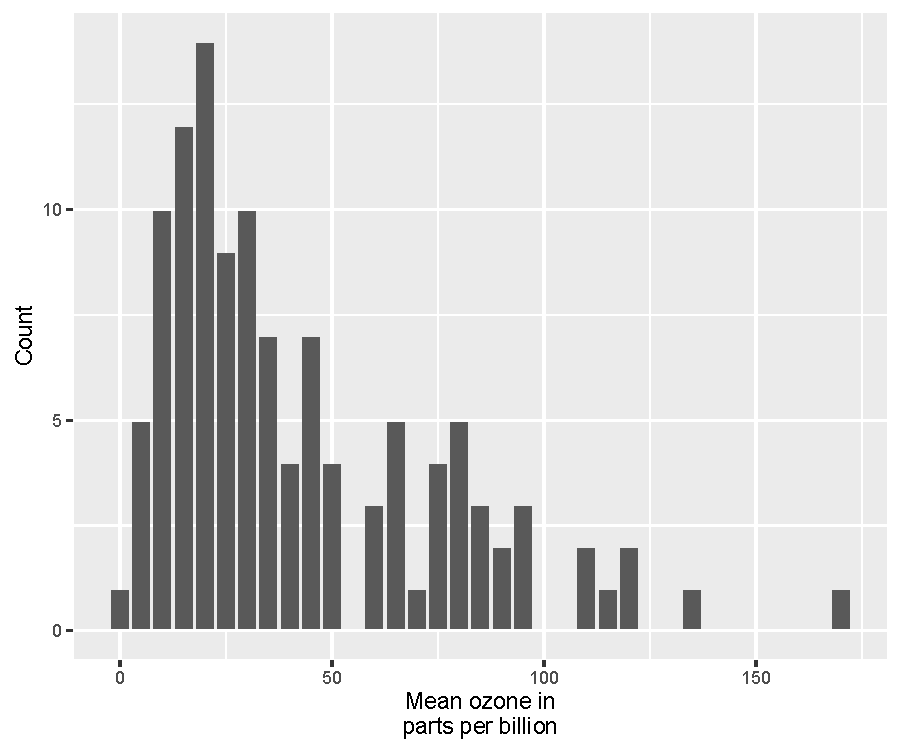
\includegraphics{7_Histograms_pdf/histogram_6-1} \end{center}

\section{Changing axis ticks}\label{changing-axis-ticks}

The next thing we will change is the axis ticks. Let's make the x-axis
ticks appear at every 25 units rather than 50 using the
\texttt{breaks\ =\ seq(0,\ 175,\ 25)} argument in
\texttt{scale\_x\_continuous}. (The \texttt{seq} function is a base R
function that indicates the start and endpoints and the units to
increment by respectively. See \texttt{help(seq)} for more information.)
We ensure that the x-axis begins and ends where we want by also adding
the argument \texttt{limits\ =\ c(0,\ 175)} to
\texttt{scale\_x\_continuous}.

\begin{Shaded}
\begin{Highlighting}[]
\NormalTok{p7 <-}\StringTok{ }\KeywordTok{ggplot}\NormalTok{(airquality, }\KeywordTok{aes}\NormalTok{(}\DataTypeTok{x =} \NormalTok{Ozone)) +}\StringTok{ }
\StringTok{  }\KeywordTok{geom_histogram}\NormalTok{(}\KeywordTok{aes}\NormalTok{(}\DataTypeTok{y =} \NormalTok{..count..), }\DataTypeTok{binwidth =} \DecValTok{5}\NormalTok{) +}
\StringTok{  }\KeywordTok{scale_x_continuous}\NormalTok{(}\DataTypeTok{name =} \StringTok{"Mean ozone in}\CharTok{\textbackslash{}n}\StringTok{parts per billion"}\NormalTok{,}
    \DataTypeTok{breaks =} \KeywordTok{seq}\NormalTok{(}\DecValTok{0}\NormalTok{, }\DecValTok{175}\NormalTok{, }\DecValTok{25}\NormalTok{), }\DataTypeTok{limits=}\KeywordTok{c}\NormalTok{(}\DecValTok{0}\NormalTok{, }\DecValTok{175}\NormalTok{)) +}
\StringTok{  }\KeywordTok{scale_y_continuous}\NormalTok{(}\DataTypeTok{name =} \StringTok{"Count"}\NormalTok{)}
\NormalTok{p7}
\end{Highlighting}
\end{Shaded}

\begin{center}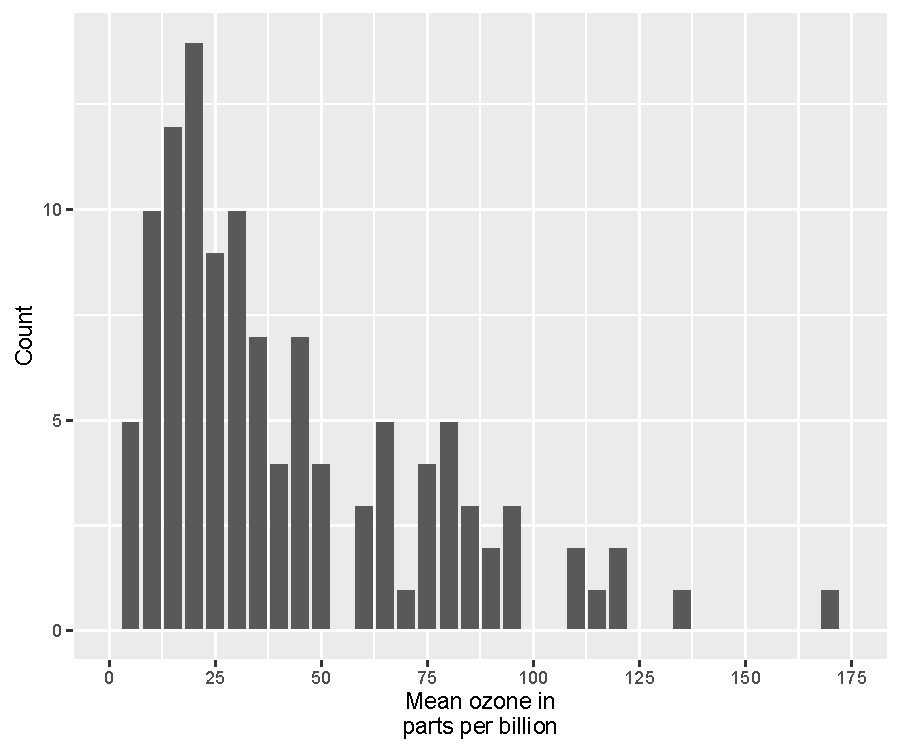
\includegraphics{7_Histograms_pdf/histogram_7-1} \end{center}

\section{Adding a title}\label{adding-a-title}

To add a title, we include the option \texttt{ggtitle} and include the
name of the graph as a string argument.

\begin{Shaded}
\begin{Highlighting}[]
\NormalTok{p7 <-}\StringTok{ }\KeywordTok{ggplot}\NormalTok{(airquality, }\KeywordTok{aes}\NormalTok{(}\DataTypeTok{x =} \NormalTok{Ozone)) +}\StringTok{ }
\StringTok{  }\KeywordTok{geom_histogram}\NormalTok{(}\KeywordTok{aes}\NormalTok{(}\DataTypeTok{y =} \NormalTok{..count..), }\DataTypeTok{binwidth =} \DecValTok{5}\NormalTok{) +}
\StringTok{  }\KeywordTok{scale_x_continuous}\NormalTok{(}\DataTypeTok{name =} \StringTok{"Mean ozone in}\CharTok{\textbackslash{}n}\StringTok{parts per billion"}\NormalTok{,}
    \DataTypeTok{breaks =} \KeywordTok{seq}\NormalTok{(}\DecValTok{0}\NormalTok{, }\DecValTok{175}\NormalTok{, }\DecValTok{25}\NormalTok{), }\DataTypeTok{limits=}\KeywordTok{c}\NormalTok{(}\DecValTok{0}\NormalTok{, }\DecValTok{175}\NormalTok{)) +}
\StringTok{  }\KeywordTok{scale_y_continuous}\NormalTok{(}\DataTypeTok{name =} \StringTok{"Count"}\NormalTok{) +}
\StringTok{  }\KeywordTok{ggtitle}\NormalTok{(}\StringTok{"Frequency histogram of mean ozone"}\NormalTok{)}
\NormalTok{p7}
\end{Highlighting}
\end{Shaded}

\begin{center}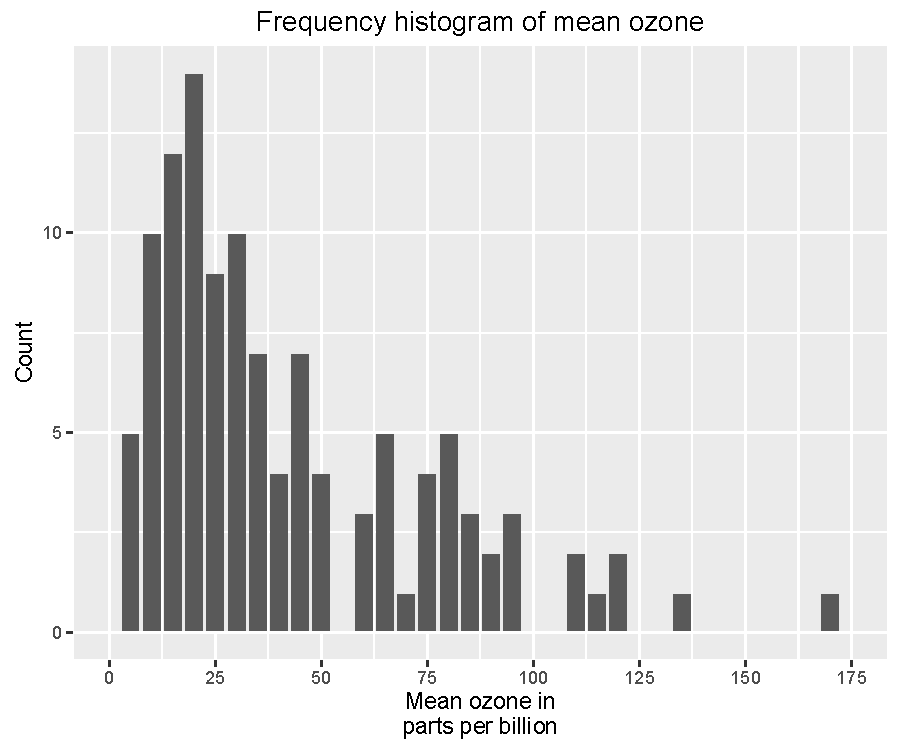
\includegraphics{7_Histograms_pdf/histogram_8-1} \end{center}

\section{Changing the colour of the
bars}\label{changing-the-colour-of-the-bars}

\subsection{By colour name}\label{by-colour-name}

To change the line and fill colours of the bars, we add a valid colour
to the \texttt{colour} and \texttt{fill} arguments in
\texttt{geom\_histogram} (note that I assigned these colours to
variables outside of the plot to make it easier to change them). A list
of valid colours is
\href{http://www.stat.columbia.edu/~tzheng/files/Rcolor.pdf}{here}.

\begin{Shaded}
\begin{Highlighting}[]
\NormalTok{barfill <-}\StringTok{ "gold1"}\NormalTok{; barlines <-}\StringTok{ "goldenrod2"}

\NormalTok{p7 <-}\StringTok{ }\KeywordTok{ggplot}\NormalTok{(airquality, }\KeywordTok{aes}\NormalTok{(}\DataTypeTok{x =} \NormalTok{Ozone)) +}\StringTok{ }
\StringTok{  }\KeywordTok{geom_histogram}\NormalTok{(}\KeywordTok{aes}\NormalTok{(}\DataTypeTok{y =} \NormalTok{..count..), }\DataTypeTok{binwidth =} \DecValTok{5}\NormalTok{,}
    \DataTypeTok{colour =} \NormalTok{barlines, }\DataTypeTok{fill =} \NormalTok{barfill) +}
\StringTok{  }\KeywordTok{scale_x_continuous}\NormalTok{(}\DataTypeTok{name =} \StringTok{"Mean ozone in}\CharTok{\textbackslash{}n}\StringTok{parts per billion"}\NormalTok{,}
    \DataTypeTok{breaks =} \KeywordTok{seq}\NormalTok{(}\DecValTok{0}\NormalTok{, }\DecValTok{175}\NormalTok{, }\DecValTok{25}\NormalTok{), }\DataTypeTok{limits=}\KeywordTok{c}\NormalTok{(}\DecValTok{0}\NormalTok{, }\DecValTok{175}\NormalTok{)) +}
\StringTok{  }\KeywordTok{scale_y_continuous}\NormalTok{(}\DataTypeTok{name =} \StringTok{"Count"}\NormalTok{) +}
\StringTok{  }\KeywordTok{ggtitle}\NormalTok{(}\StringTok{"Frequency histogram of mean ozone"}\NormalTok{)}
\NormalTok{p7}
\end{Highlighting}
\end{Shaded}

\begin{center}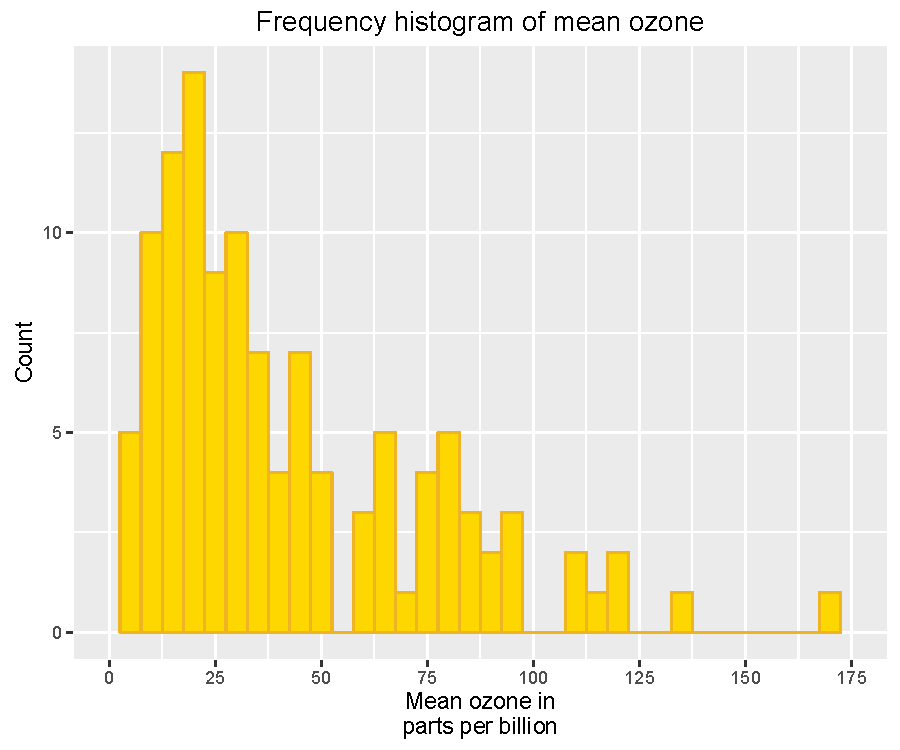
\includegraphics{7_Histograms_pdf/histogram_9-1} \end{center}

\subsection{By HEX code}\label{by-hex-code}

If you want to go beyond the options in the list above, you can also
specify exact HEX colours by including them as a string preceded by a
hash, e.g., ``\#FFFFFF''. Below, we have called two shades of blue for
the fill and lines using their HEX codes.

\begin{Shaded}
\begin{Highlighting}[]
\NormalTok{barfill <-}\StringTok{ "#4271AE"}\NormalTok{; barlines <-}\StringTok{ "#1F3552"}

\NormalTok{p7 <-}\StringTok{ }\KeywordTok{ggplot}\NormalTok{(airquality, }\KeywordTok{aes}\NormalTok{(}\DataTypeTok{x =} \NormalTok{Ozone)) +}\StringTok{ }
\StringTok{  }\KeywordTok{geom_histogram}\NormalTok{(}\KeywordTok{aes}\NormalTok{(}\DataTypeTok{y =} \NormalTok{..count..), }\DataTypeTok{binwidth =} \DecValTok{5}\NormalTok{,}
    \DataTypeTok{colour =} \NormalTok{barlines, }\DataTypeTok{fill =} \NormalTok{barfill) +}
\StringTok{  }\KeywordTok{scale_x_continuous}\NormalTok{(}\DataTypeTok{name =} \StringTok{"Mean ozone in}\CharTok{\textbackslash{}n}\StringTok{parts per billion"}\NormalTok{,}
    \DataTypeTok{breaks =} \KeywordTok{seq}\NormalTok{(}\DecValTok{0}\NormalTok{, }\DecValTok{175}\NormalTok{, }\DecValTok{25}\NormalTok{), }\DataTypeTok{limits=}\KeywordTok{c}\NormalTok{(}\DecValTok{0}\NormalTok{, }\DecValTok{175}\NormalTok{)) +}
\StringTok{  }\KeywordTok{scale_y_continuous}\NormalTok{(}\DataTypeTok{name =} \StringTok{"Count"}\NormalTok{) +}
\StringTok{  }\KeywordTok{ggtitle}\NormalTok{(}\StringTok{"Frequency histogram of mean ozone"}\NormalTok{)}
\NormalTok{p7}
\end{Highlighting}
\end{Shaded}

\begin{center}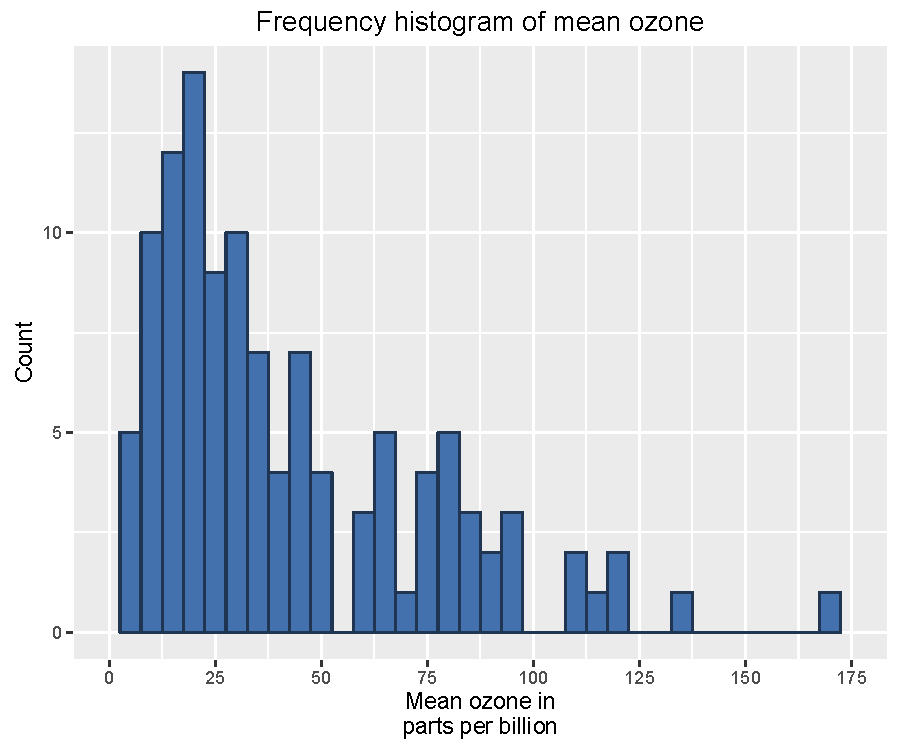
\includegraphics{7_Histograms_pdf/histogram_10-1} \end{center}

\section{Colour gradients}\label{colour-gradients}

You can also add a gradient to your colour scheme that varies according
to the frequency of the values. Below is the default gradient colour
scheme. In order to do this, you can see we have changed the
\texttt{aes(y\ =\ ..count..)} argument in \texttt{geom\_histogram} to
\texttt{aes(fill\ =\ ..count..)}.

\begin{Shaded}
\begin{Highlighting}[]
\NormalTok{p7 <-}\StringTok{ }\KeywordTok{ggplot}\NormalTok{(airquality, }\KeywordTok{aes}\NormalTok{(}\DataTypeTok{x =} \NormalTok{Ozone)) +}\StringTok{ }
\StringTok{  }\KeywordTok{geom_histogram}\NormalTok{(}\KeywordTok{aes}\NormalTok{(}\DataTypeTok{fill =} \NormalTok{..count..), }\DataTypeTok{binwidth =} \DecValTok{5}\NormalTok{) +}
\StringTok{  }\KeywordTok{scale_x_continuous}\NormalTok{(}\DataTypeTok{name =} \StringTok{"Mean ozone in}\CharTok{\textbackslash{}n}\StringTok{parts per billion"}\NormalTok{,}
    \DataTypeTok{breaks =} \KeywordTok{seq}\NormalTok{(}\DecValTok{0}\NormalTok{, }\DecValTok{175}\NormalTok{, }\DecValTok{25}\NormalTok{), }\DataTypeTok{limits=}\KeywordTok{c}\NormalTok{(}\DecValTok{0}\NormalTok{, }\DecValTok{175}\NormalTok{)) +}
\StringTok{  }\KeywordTok{scale_y_continuous}\NormalTok{(}\DataTypeTok{name =} \StringTok{"Count"}\NormalTok{) +}
\StringTok{  }\KeywordTok{ggtitle}\NormalTok{(}\StringTok{"Frequency histogram of mean ozone"}\NormalTok{)}
\NormalTok{p7}
\end{Highlighting}
\end{Shaded}

\begin{center}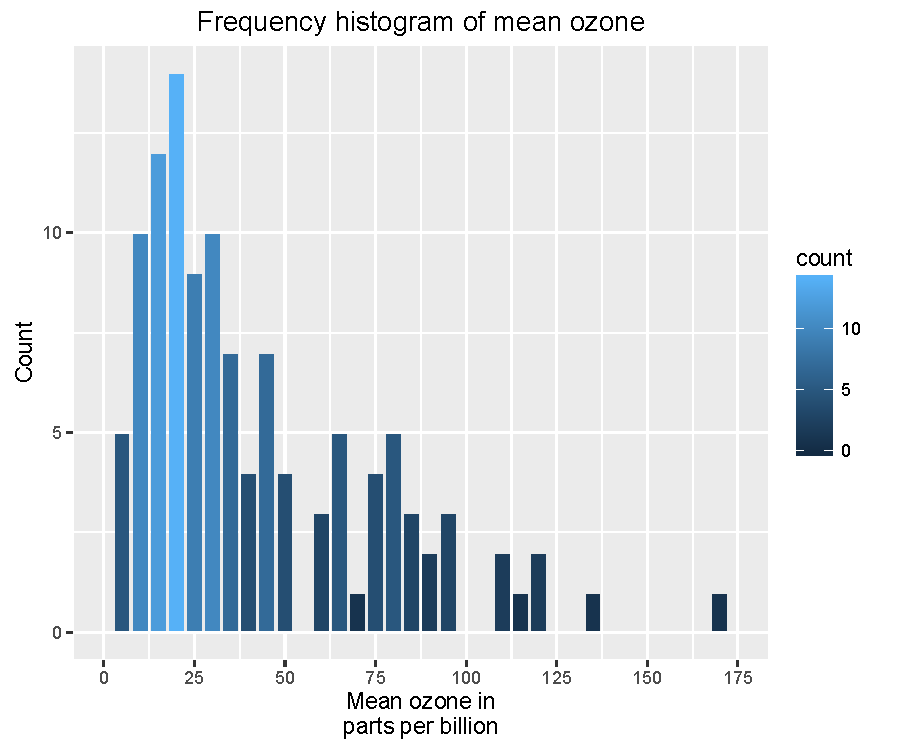
\includegraphics{7_Histograms_pdf/histogram_11-1} \end{center}

You can customise the gradient by changing the anchoring colours for
high and low. To do so, we have added the option
\texttt{scale\_fill\_gradient} to the plot with the arguments
\texttt{Count} (the name of the legend), \texttt{low} (the colour for
the least frequent values) and \texttt{high} (the colour for the most
frequent values).

\begin{Shaded}
\begin{Highlighting}[]
\NormalTok{p7 <-}\StringTok{ }\KeywordTok{ggplot}\NormalTok{(airquality, }\KeywordTok{aes}\NormalTok{(}\DataTypeTok{x =} \NormalTok{Ozone)) +}\StringTok{ }
\StringTok{  }\KeywordTok{geom_histogram}\NormalTok{(}\KeywordTok{aes}\NormalTok{(}\DataTypeTok{fill =} \NormalTok{..count..), }\DataTypeTok{binwidth =} \DecValTok{5}\NormalTok{) +}
\StringTok{  }\KeywordTok{scale_x_continuous}\NormalTok{(}\DataTypeTok{name =} \StringTok{"Mean ozone in}\CharTok{\textbackslash{}n}\StringTok{parts per billion"}\NormalTok{,}
    \DataTypeTok{breaks =} \KeywordTok{seq}\NormalTok{(}\DecValTok{0}\NormalTok{, }\DecValTok{175}\NormalTok{, }\DecValTok{25}\NormalTok{), }\DataTypeTok{limits=}\KeywordTok{c}\NormalTok{(}\DecValTok{0}\NormalTok{, }\DecValTok{175}\NormalTok{)) +}
\StringTok{  }\KeywordTok{scale_y_continuous}\NormalTok{(}\DataTypeTok{name =} \StringTok{"Count"}\NormalTok{) +}
\StringTok{  }\KeywordTok{ggtitle}\NormalTok{(}\StringTok{"Frequency histogram of mean ozone"}\NormalTok{) +}
\StringTok{  }\KeywordTok{scale_fill_gradient}\NormalTok{(}\StringTok{"Count"}\NormalTok{, }\DataTypeTok{low =} \StringTok{"blue"}\NormalTok{, }\DataTypeTok{high =} \StringTok{"red"}\NormalTok{)}
\NormalTok{p7}
\end{Highlighting}
\end{Shaded}

\begin{center}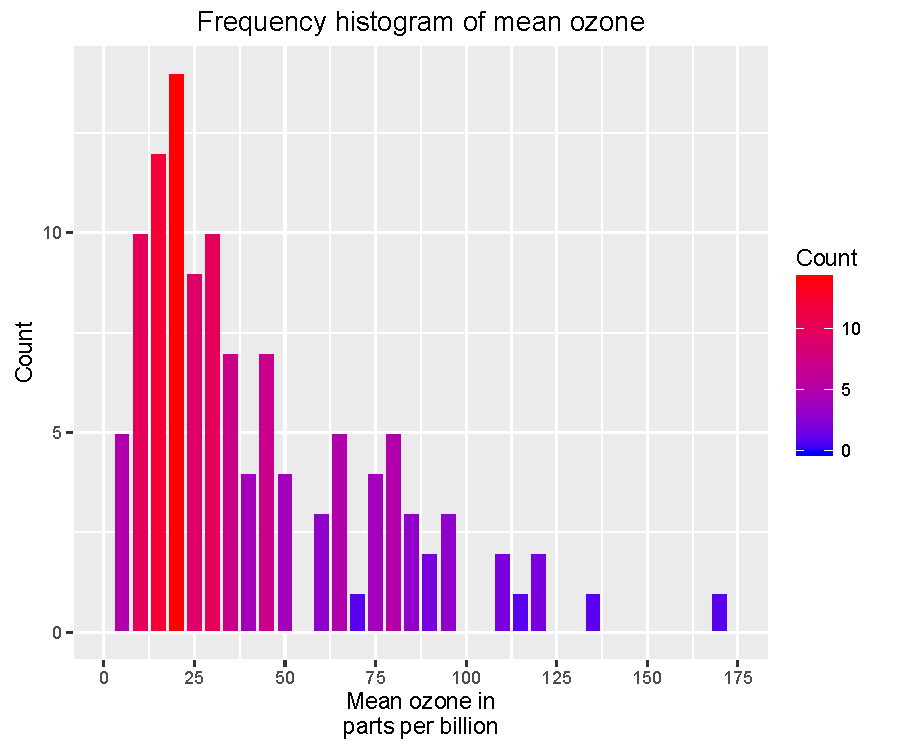
\includegraphics{7_Histograms_pdf/histogram_12-1} \end{center}

\section{Using the white theme}\label{using-the-white-theme}

As explained in the previous posts, we can also change the overall look
of the plot using themes. We'll start using a simple theme customisation
by adding \texttt{theme\_bw()} after \texttt{ggplot()}. As you can see,
we can further tweak the graph using the \texttt{theme} option, which
we've used so far to change the legend.

\begin{Shaded}
\begin{Highlighting}[]
\NormalTok{p7 <-}\StringTok{ }\KeywordTok{ggplot}\NormalTok{(airquality, }\KeywordTok{aes}\NormalTok{(}\DataTypeTok{x =} \NormalTok{Ozone)) +}\StringTok{ }
\StringTok{  }\KeywordTok{geom_histogram}\NormalTok{(}\KeywordTok{aes}\NormalTok{(}\DataTypeTok{y =} \NormalTok{..count..), }\DataTypeTok{binwidth =} \DecValTok{5}\NormalTok{,}
  \DataTypeTok{colour =} \NormalTok{barlines, }\DataTypeTok{fill =} \NormalTok{barfill) +}
\StringTok{    }\KeywordTok{scale_x_continuous}\NormalTok{(}\DataTypeTok{name =} \StringTok{"Mean ozone in}\CharTok{\textbackslash{}n}\StringTok{parts per billion"}\NormalTok{,}
    \DataTypeTok{breaks =} \KeywordTok{seq}\NormalTok{(}\DecValTok{0}\NormalTok{, }\DecValTok{175}\NormalTok{, }\DecValTok{25}\NormalTok{),}
    \DataTypeTok{limits=}\KeywordTok{c}\NormalTok{(}\DecValTok{0}\NormalTok{, }\DecValTok{175}\NormalTok{)) +}
\StringTok{    }\KeywordTok{scale_y_continuous}\NormalTok{(}\DataTypeTok{name =} \StringTok{"Count"}\NormalTok{) +}
\StringTok{  }\KeywordTok{ggtitle}\NormalTok{(}\StringTok{"Frequency histogram of mean ozone"}\NormalTok{) +}
\StringTok{  }\KeywordTok{theme_bw}\NormalTok{()}
\NormalTok{p7}
\end{Highlighting}
\end{Shaded}

\begin{center}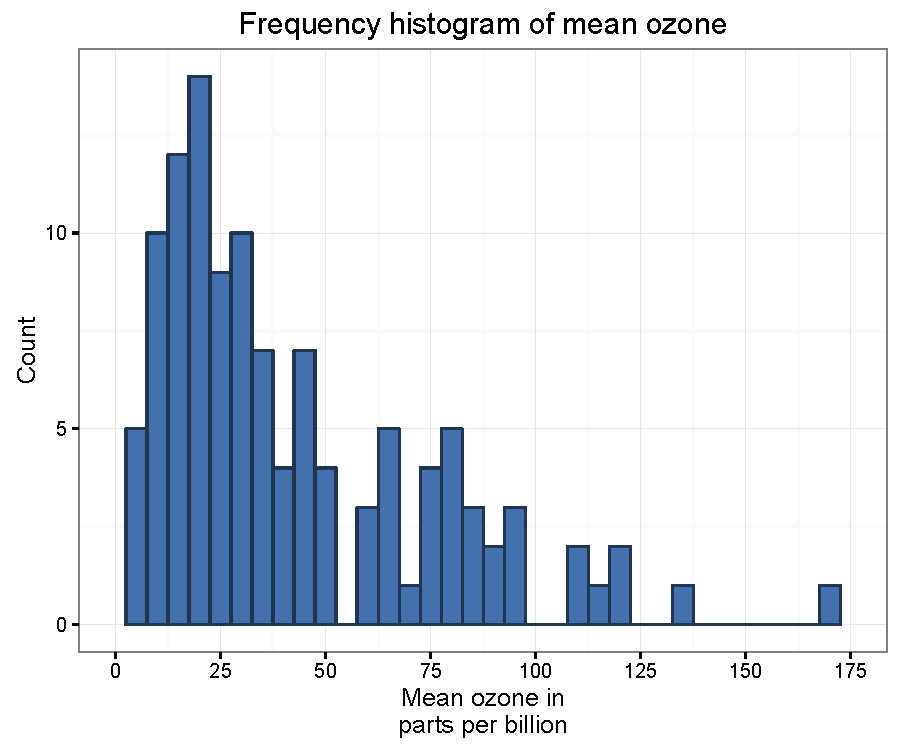
\includegraphics{7_Histograms_pdf/histogram_13-1} \end{center}

\section{Creating an XKCD style
chart}\label{creating-an-xkcd-style-chart}

Of course, you may want to create your own themes as well.
\texttt{ggplot2} allows for a very high degree of customisation,
including allowing you to use imported fonts. Below is an example of a
theme Mauricio was able to create which mimics the visual style of
\href{http://xkcd.com/}{XKCD}. In order to create this chart, you first
need to import the XKCD font, and load it into R using the
\texttt{extrafont} package.

\begin{Shaded}
\begin{Highlighting}[]
\NormalTok{p7 <-}\StringTok{ }\KeywordTok{ggplot}\NormalTok{(airquality, }\KeywordTok{aes}\NormalTok{(}\DataTypeTok{x =} \NormalTok{Ozone)) +}\StringTok{ }
\StringTok{  }\KeywordTok{geom_histogram}\NormalTok{(}\KeywordTok{aes}\NormalTok{(}\DataTypeTok{y =} \NormalTok{..count..), }\DataTypeTok{binwidth =} \DecValTok{10}\NormalTok{,}
    \DataTypeTok{colour =} \StringTok{"black"}\NormalTok{, }\DataTypeTok{fill =} \StringTok{"#56B4E9"}\NormalTok{) +}
\StringTok{  }\KeywordTok{scale_x_continuous}\NormalTok{(}\DataTypeTok{name =} \StringTok{"Mean ozone in}\CharTok{\textbackslash{}n}\StringTok{parts per billion"}\NormalTok{,}
    \DataTypeTok{breaks =} \KeywordTok{seq}\NormalTok{(}\DecValTok{0}\NormalTok{, }\DecValTok{175}\NormalTok{, }\DecValTok{25}\NormalTok{), }\DataTypeTok{limits=}\KeywordTok{c}\NormalTok{(}\DecValTok{0}\NormalTok{, }\DecValTok{175}\NormalTok{)) +}
\StringTok{  }\KeywordTok{scale_y_continuous}\NormalTok{(}\DataTypeTok{name =} \StringTok{"Count"}\NormalTok{) +}
\StringTok{  }\KeywordTok{ggtitle}\NormalTok{(}\StringTok{"Frequency histogram of mean ozone"}\NormalTok{) +}\StringTok{ }
\StringTok{  }\KeywordTok{theme}\NormalTok{(}\DataTypeTok{axis.line.x =} \KeywordTok{element_line}\NormalTok{(}\DataTypeTok{size=}\NormalTok{.}\DecValTok{5}\NormalTok{, }\DataTypeTok{colour =} \StringTok{"black"}\NormalTok{), }
    \DataTypeTok{axis.line.y =} \KeywordTok{element_line}\NormalTok{(}\DataTypeTok{size=}\NormalTok{.}\DecValTok{5}\NormalTok{, }\DataTypeTok{colour =} \StringTok{"black"}\NormalTok{),     }
    \DataTypeTok{axis.text.x=}\KeywordTok{element_text}\NormalTok{(}\DataTypeTok{colour=}\StringTok{"black"}\NormalTok{, }\DataTypeTok{size =} \DecValTok{10}\NormalTok{), }
    \DataTypeTok{axis.text.y=}\KeywordTok{element_text}\NormalTok{(}\DataTypeTok{colour=}\StringTok{"black"}\NormalTok{, }\DataTypeTok{size =} \DecValTok{10}\NormalTok{), }
    \DataTypeTok{legend.position=}\StringTok{"bottom"}\NormalTok{, }
    \DataTypeTok{legend.direction=}\StringTok{"horizontal"}\NormalTok{,}
    \DataTypeTok{legend.box =} \StringTok{"horizontal"}\NormalTok{, }
    \DataTypeTok{legend.key.size =} \KeywordTok{unit}\NormalTok{(}\DecValTok{1}\NormalTok{, }\StringTok{"cm"}\NormalTok{),}
    \DataTypeTok{legend.key =} \KeywordTok{element_blank}\NormalTok{(),}
    \DataTypeTok{panel.grid.major =} \KeywordTok{element_blank}\NormalTok{(),}
    \DataTypeTok{panel.grid.minor =} \KeywordTok{element_blank}\NormalTok{(), }
    \DataTypeTok{panel.border =} \KeywordTok{element_blank}\NormalTok{(),}
    \DataTypeTok{panel.background =} \KeywordTok{element_blank}\NormalTok{(),}
    \DataTypeTok{plot.title=}\KeywordTok{element_text}\NormalTok{(}\DataTypeTok{family=}\StringTok{"xkcd-Regular"}\NormalTok{), }
    \DataTypeTok{text=}\KeywordTok{element_text}\NormalTok{(}\DataTypeTok{family=}\StringTok{"xkcd-Regular"}\NormalTok{)) }
\NormalTok{p7}
\end{Highlighting}
\end{Shaded}

\begin{center}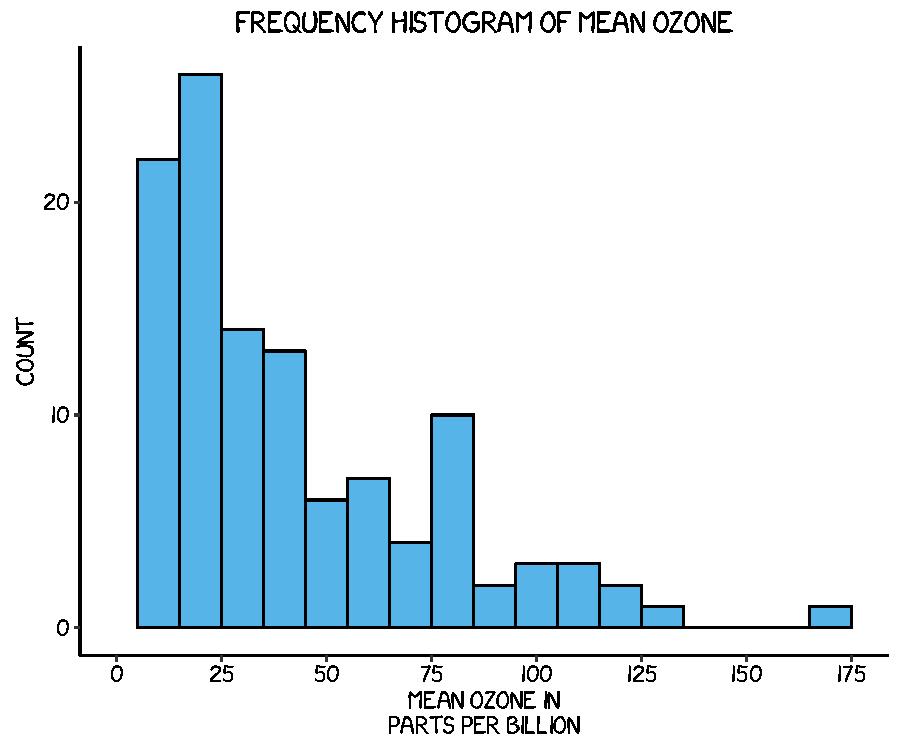
\includegraphics{7_Histograms_pdf/histogram_14-1} \end{center}

\section{\texorpdfstring{Using `The Economist'
theme}{Using The Economist theme}}\label{using-the-economist-theme}

There are a wider range of pre-built themes available as part of the
\texttt{ggthemes} package (more information on these
\href{https://cran.r-project.org/web/packages/ggthemes/vignettes/ggthemes.html}{here}).
Below we've applied \texttt{theme\_economist()}, which approximates
graphs in the Economist magazine.

\begin{Shaded}
\begin{Highlighting}[]
\NormalTok{p7 <-}\StringTok{ }\KeywordTok{ggplot}\NormalTok{(airquality, }\KeywordTok{aes}\NormalTok{(}\DataTypeTok{x =} \NormalTok{Ozone)) +}\StringTok{ }
\StringTok{  }\KeywordTok{geom_histogram}\NormalTok{(}\KeywordTok{aes}\NormalTok{(}\DataTypeTok{y =} \NormalTok{..count..), }\DataTypeTok{binwidth =} \DecValTok{5}\NormalTok{, }
    \DataTypeTok{colour =} \NormalTok{barlines, }\DataTypeTok{fill =} \NormalTok{barfill) +}
\StringTok{  }\KeywordTok{scale_x_continuous}\NormalTok{(}\DataTypeTok{name =} \StringTok{"Mean ozone in}\CharTok{\textbackslash{}n}\StringTok{parts per billion"}\NormalTok{,}
    \DataTypeTok{breaks =} \KeywordTok{seq}\NormalTok{(}\DecValTok{0}\NormalTok{, }\DecValTok{175}\NormalTok{, }\DecValTok{25}\NormalTok{), }\DataTypeTok{limits=}\KeywordTok{c}\NormalTok{(}\DecValTok{0}\NormalTok{, }\DecValTok{175}\NormalTok{)) +}
\StringTok{  }\KeywordTok{scale_y_continuous}\NormalTok{(}\DataTypeTok{name =} \StringTok{"Count"}\NormalTok{) +}
\StringTok{  }\KeywordTok{ggtitle}\NormalTok{(}\StringTok{"Frequency histogram of mean ozone"}\NormalTok{) +}
\StringTok{  }\KeywordTok{theme_economist}\NormalTok{() +}\StringTok{ }\KeywordTok{scale_fill_economist}\NormalTok{() +}
\StringTok{  }\KeywordTok{theme}\NormalTok{(}\DataTypeTok{axis.line.x =} \KeywordTok{element_line}\NormalTok{(}\DataTypeTok{size=}\NormalTok{.}\DecValTok{5}\NormalTok{, }\DataTypeTok{colour =} \StringTok{"black"}\NormalTok{),}
    \DataTypeTok{axis.title =} \KeywordTok{element_text}\NormalTok{(}\DataTypeTok{size =} \DecValTok{12}\NormalTok{),}
    \DataTypeTok{legend.position=}\StringTok{"bottom"}\NormalTok{, }
    \DataTypeTok{legend.direction=}\StringTok{"horizontal"}\NormalTok{,}
    \DataTypeTok{legend.box =} \StringTok{"horizontal"}\NormalTok{, }
    \DataTypeTok{legend.key.size =} \KeywordTok{unit}\NormalTok{(}\DecValTok{1}\NormalTok{, }\StringTok{"cm"}\NormalTok{),}
    \DataTypeTok{legend.text =} \KeywordTok{element_text}\NormalTok{(}\DataTypeTok{size =} \DecValTok{10}\NormalTok{),}
    \DataTypeTok{text =} \KeywordTok{element_text}\NormalTok{(}\DataTypeTok{family =} \StringTok{"OfficinaSanITC-Book"}\NormalTok{),}
    \DataTypeTok{plot.title =} \KeywordTok{element_text}\NormalTok{(}\DataTypeTok{family=}\StringTok{"OfficinaSanITC-Book"}\NormalTok{))}
\NormalTok{p7}
\end{Highlighting}
\end{Shaded}

\begin{center}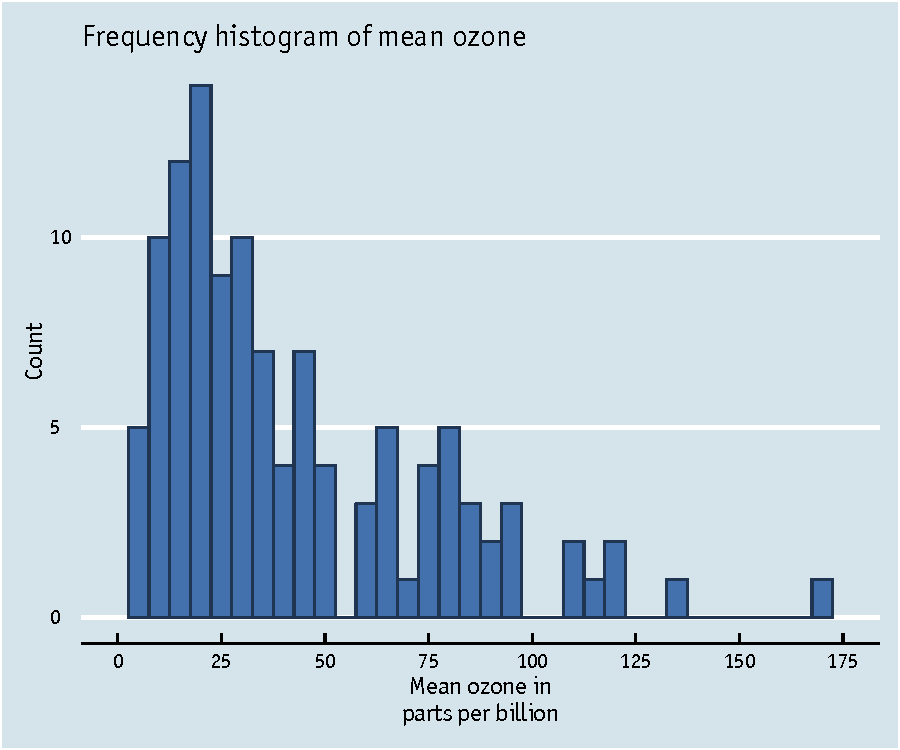
\includegraphics{7_Histograms_pdf/histogram_15-1} \end{center}

\section{\texorpdfstring{Using `Five Thirty Eight'
theme}{Using Five Thirty Eight theme}}\label{using-five-thirty-eight-theme}

Below we've applied \texttt{theme\_fivethirtyeight()}, which
approximates graphs in the nice
\href{http://fivethirtyeight.com/}{FiveThirtyEight} website. Again, it
is also important that the font change is optional and it's only to
obtain a more similar result compared to the original. For an exact
result you need `Atlas Grotesk' and `Decima Mono Pro' which are
commercial font and are available
\href{https://commercialtype.com/catalog/atlas}{here} and
\href{https://www.myfonts.com/fonts/tipografiaramis/decima-mono-pro/}{here}.

\begin{Shaded}
\begin{Highlighting}[]
\NormalTok{p7 <-}\StringTok{ }\KeywordTok{ggplot}\NormalTok{(airquality, }\KeywordTok{aes}\NormalTok{(}\DataTypeTok{x =} \NormalTok{Ozone)) +}\StringTok{ }
\StringTok{  }\KeywordTok{geom_histogram}\NormalTok{(}\KeywordTok{aes}\NormalTok{(}\DataTypeTok{y =} \NormalTok{..count..), }\DataTypeTok{binwidth =} \DecValTok{5}\NormalTok{, }
    \DataTypeTok{colour =} \NormalTok{barlines, }\DataTypeTok{fill =} \NormalTok{barfill) +}
\StringTok{  }\KeywordTok{scale_x_continuous}\NormalTok{(}\DataTypeTok{name =} \StringTok{"Mean ozone in}\CharTok{\textbackslash{}n}\StringTok{parts per billion"}\NormalTok{,}
    \DataTypeTok{breaks =} \KeywordTok{seq}\NormalTok{(}\DecValTok{0}\NormalTok{, }\DecValTok{175}\NormalTok{, }\DecValTok{25}\NormalTok{), }\DataTypeTok{limits=}\KeywordTok{c}\NormalTok{(}\DecValTok{0}\NormalTok{, }\DecValTok{175}\NormalTok{)) +}
\StringTok{  }\KeywordTok{scale_y_continuous}\NormalTok{(}\DataTypeTok{name =} \StringTok{"Count"}\NormalTok{) +}
\StringTok{  }\KeywordTok{ggtitle}\NormalTok{(}\StringTok{"Frequency histogram of mean ozone"}\NormalTok{) +}
\StringTok{  }\KeywordTok{theme_fivethirtyeight}\NormalTok{() +}\StringTok{ }\KeywordTok{scale_fill_fivethirtyeight}\NormalTok{() +}\StringTok{   }
\StringTok{  }\KeywordTok{theme}\NormalTok{(}\DataTypeTok{axis.title =} \KeywordTok{element_text}\NormalTok{(}\DataTypeTok{family=}\StringTok{"Atlas Grotesk Regular"}\NormalTok{),}
    \DataTypeTok{legend.position=}\StringTok{"bottom"}\NormalTok{, }
    \DataTypeTok{legend.direction=}\StringTok{"horizontal"}\NormalTok{,}
    \DataTypeTok{legend.box =} \StringTok{"horizontal"}\NormalTok{, }
    \DataTypeTok{legend.key.size =} \KeywordTok{unit}\NormalTok{(}\DecValTok{1}\NormalTok{, }\StringTok{"cm"}\NormalTok{),}
    \DataTypeTok{legend.title=}\KeywordTok{element_text}\NormalTok{(}\DataTypeTok{family=}\StringTok{"Atlas Grotesk Regular"}\NormalTok{, }\DataTypeTok{size =} \DecValTok{10}\NormalTok{),}
    \DataTypeTok{legend.text=}\KeywordTok{element_text}\NormalTok{(}\DataTypeTok{family=}\StringTok{"Atlas Grotesk Regular"}\NormalTok{, }\DataTypeTok{size =} \DecValTok{10}\NormalTok{),}
    \DataTypeTok{plot.title=}\KeywordTok{element_text}\NormalTok{(}\DataTypeTok{family=}\StringTok{"Atlas Grotesk Medium"}\NormalTok{), }
    \DataTypeTok{text=}\KeywordTok{element_text}\NormalTok{(}\DataTypeTok{family=}\StringTok{"DecimaMonoPro"}\NormalTok{)) }
\NormalTok{p7}
\end{Highlighting}
\end{Shaded}

\begin{center}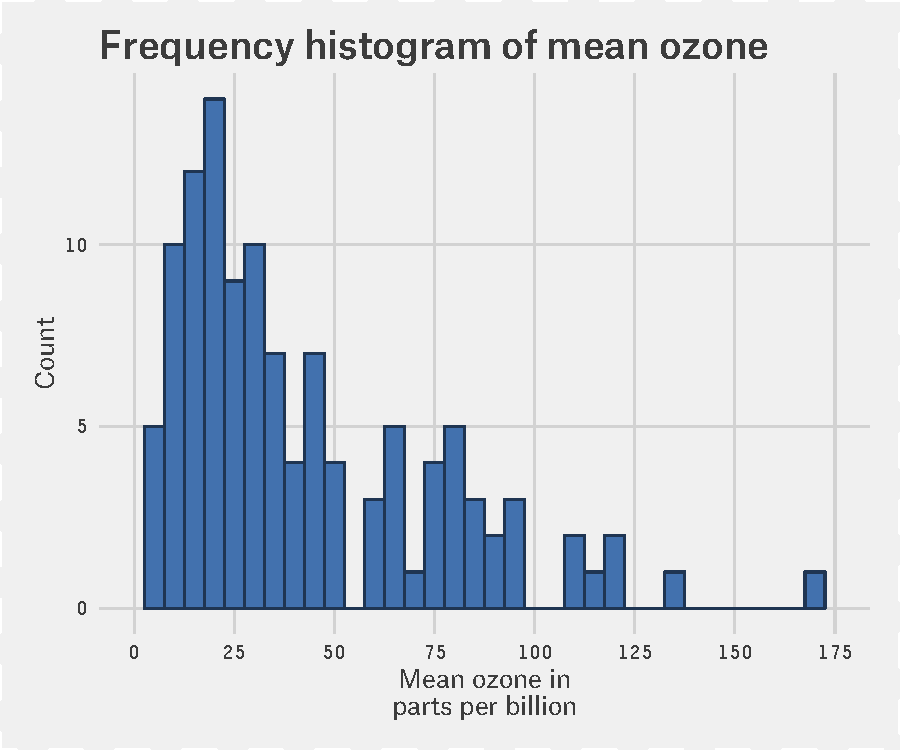
\includegraphics{7_Histograms_pdf/histogram_16-1} \end{center}

\section{Creating your own theme}\label{creating-your-own-theme}

As before, you can modify your plots a lot as \texttt{ggplot2} allows
many customisations. Here is a custom plot where we have modified the
axes, background and font.

\begin{Shaded}
\begin{Highlighting}[]
\NormalTok{barfill <-}\StringTok{ "#4271AE"}\NormalTok{; barlines <-}\StringTok{ "#1F3552"}

\NormalTok{p7 <-}\StringTok{ }\KeywordTok{ggplot}\NormalTok{(airquality, }\KeywordTok{aes}\NormalTok{(}\DataTypeTok{x =} \NormalTok{Ozone)) +}\StringTok{ }
\StringTok{  }\KeywordTok{geom_histogram}\NormalTok{(}\KeywordTok{aes}\NormalTok{(}\DataTypeTok{y =} \NormalTok{..count..), }\DataTypeTok{binwidth =} \DecValTok{5}\NormalTok{, }
    \DataTypeTok{colour =} \NormalTok{barlines, }\DataTypeTok{fill =} \NormalTok{barfill) +}
\StringTok{  }\KeywordTok{scale_x_continuous}\NormalTok{(}\DataTypeTok{name =} \StringTok{"Mean ozone in}\CharTok{\textbackslash{}n}\StringTok{parts per billion"}\NormalTok{,}
    \DataTypeTok{breaks =} \KeywordTok{seq}\NormalTok{(}\DecValTok{0}\NormalTok{, }\DecValTok{175}\NormalTok{, }\DecValTok{25}\NormalTok{),}
    \DataTypeTok{limits=}\KeywordTok{c}\NormalTok{(}\DecValTok{0}\NormalTok{, }\DecValTok{175}\NormalTok{)) +}
\StringTok{  }\KeywordTok{scale_y_continuous}\NormalTok{(}\DataTypeTok{name =} \StringTok{"Count"}\NormalTok{) +}
\StringTok{  }\KeywordTok{ggtitle}\NormalTok{(}\StringTok{"Frequency histogram of mean ozone"}\NormalTok{) +}
\StringTok{  }\KeywordTok{theme}\NormalTok{(}\DataTypeTok{panel.border =} \KeywordTok{element_rect}\NormalTok{(}\DataTypeTok{colour =} \StringTok{"black"}\NormalTok{, }\DataTypeTok{fill=}\OtherTok{NA}\NormalTok{, }\DataTypeTok{size=}\NormalTok{.}\DecValTok{5}\NormalTok{), }
    \DataTypeTok{axis.text.x=}\KeywordTok{element_text}\NormalTok{(}\DataTypeTok{colour=}\StringTok{"black"}\NormalTok{, }\DataTypeTok{size =} \DecValTok{9}\NormalTok{), }
    \DataTypeTok{axis.text.y=}\KeywordTok{element_text}\NormalTok{(}\DataTypeTok{colour=}\StringTok{"black"}\NormalTok{, }\DataTypeTok{size =} \DecValTok{9}\NormalTok{),}
    \DataTypeTok{legend.position=}\StringTok{"bottom"}\NormalTok{, }
    \DataTypeTok{legend.direction=}\StringTok{"horizontal"}\NormalTok{,}
    \DataTypeTok{legend.box =} \StringTok{"horizontal"}\NormalTok{, }
    \DataTypeTok{legend.key.size =} \KeywordTok{unit}\NormalTok{(}\DecValTok{1}\NormalTok{, }\StringTok{"cm"}\NormalTok{),}
    \DataTypeTok{legend.key =} \KeywordTok{element_blank}\NormalTok{(),}
    \DataTypeTok{panel.grid.major =} \KeywordTok{element_line}\NormalTok{(}\DataTypeTok{colour =} \StringTok{"#d3d3d3"}\NormalTok{), }
    \DataTypeTok{panel.grid.minor =} \KeywordTok{element_blank}\NormalTok{(), }
    \DataTypeTok{panel.border =} \KeywordTok{element_blank}\NormalTok{(), }\DataTypeTok{panel.background =} \KeywordTok{element_blank}\NormalTok{(),}
    \DataTypeTok{plot.title =} \KeywordTok{element_text}\NormalTok{(}\DataTypeTok{size =} \DecValTok{14}\NormalTok{, }\DataTypeTok{family =} \StringTok{"Tahoma"}\NormalTok{, }\DataTypeTok{face =} \StringTok{"bold"}\NormalTok{),}
    \DataTypeTok{text=}\KeywordTok{element_text}\NormalTok{(}\DataTypeTok{family=}\StringTok{"Tahoma"}\NormalTok{)) }
\NormalTok{p7}
\end{Highlighting}
\end{Shaded}

\begin{center}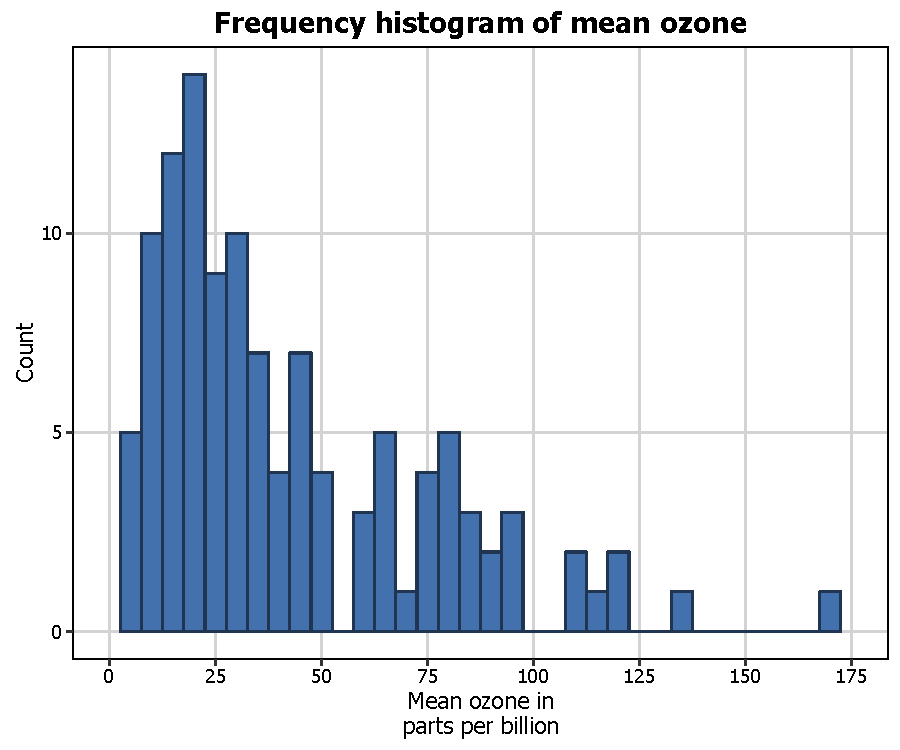
\includegraphics{7_Histograms_pdf/histogram_17-1} \end{center}

\section{Adding lines}\label{adding-lines}

Let's say that we want to add a cutoff value to the chart (75 parts of
ozone per billion). We add the \texttt{geom\_vline} option to the chart,
and specify where it goes on the x-axis using the \texttt{xintercept}
argument. We can customise how it looks using the \texttt{colour} and
\texttt{linetype} arguments in \texttt{geom\_vline}. (In the the same
way, horizontal lines can be added using the \texttt{geom\_hline}.)

\begin{Shaded}
\begin{Highlighting}[]
\NormalTok{barfill <-}\StringTok{ "#4271AE"}\NormalTok{; barlines <-}\StringTok{ "#1F3552"}

\NormalTok{p7 <-}\StringTok{ }\KeywordTok{ggplot}\NormalTok{(airquality, }\KeywordTok{aes}\NormalTok{(}\DataTypeTok{x =} \NormalTok{Ozone)) +}\StringTok{ }
\StringTok{  }\KeywordTok{geom_histogram}\NormalTok{(}\KeywordTok{aes}\NormalTok{(}\DataTypeTok{y =} \NormalTok{..count..), }\DataTypeTok{binwidth =} \DecValTok{5}\NormalTok{,}
    \DataTypeTok{colour =} \NormalTok{barlines, }\DataTypeTok{fill =} \NormalTok{barfill) +}
\StringTok{  }\KeywordTok{scale_x_continuous}\NormalTok{(}\DataTypeTok{name =} \StringTok{"Mean ozone in}\CharTok{\textbackslash{}n}\StringTok{parts per billion"}\NormalTok{,}
    \DataTypeTok{breaks =} \KeywordTok{seq}\NormalTok{(}\DecValTok{0}\NormalTok{, }\DecValTok{175}\NormalTok{, }\DecValTok{25}\NormalTok{), }\DataTypeTok{limits=}\KeywordTok{c}\NormalTok{(}\DecValTok{0}\NormalTok{, }\DecValTok{175}\NormalTok{)) +}
\StringTok{  }\KeywordTok{scale_y_continuous}\NormalTok{(}\DataTypeTok{name =} \StringTok{"Count"}\NormalTok{) +}
\StringTok{  }\KeywordTok{ggtitle}\NormalTok{(}\StringTok{"Frequency histogram of mean ozone"}\NormalTok{) +}
\StringTok{  }\KeywordTok{geom_vline}\NormalTok{(}\DataTypeTok{xintercept =} \DecValTok{75}\NormalTok{, }\DataTypeTok{size =} \DecValTok{1}\NormalTok{, }\DataTypeTok{colour =} \StringTok{"#FF3721"}\NormalTok{, }
    \DataTypeTok{linetype =} \StringTok{"dashed"}\NormalTok{) +}
\StringTok{  }\KeywordTok{theme}\NormalTok{(}\DataTypeTok{panel.border =} \KeywordTok{element_rect}\NormalTok{(}\DataTypeTok{colour =} \StringTok{"black"}\NormalTok{, }\DataTypeTok{fill=}\OtherTok{NA}\NormalTok{, }\DataTypeTok{size=}\NormalTok{.}\DecValTok{5}\NormalTok{), }
    \DataTypeTok{axis.text.x=}\KeywordTok{element_text}\NormalTok{(}\DataTypeTok{colour=}\StringTok{"black"}\NormalTok{, }\DataTypeTok{size =} \DecValTok{9}\NormalTok{), }
    \DataTypeTok{axis.text.y=}\KeywordTok{element_text}\NormalTok{(}\DataTypeTok{colour=}\StringTok{"black"}\NormalTok{, }\DataTypeTok{size =} \DecValTok{9}\NormalTok{),}
    \DataTypeTok{legend.position=}\StringTok{"bottom"}\NormalTok{, }
    \DataTypeTok{legend.direction=}\StringTok{"horizontal"}\NormalTok{,}
    \DataTypeTok{legend.box =} \StringTok{"horizontal"}\NormalTok{, }
    \DataTypeTok{legend.key.size =} \KeywordTok{unit}\NormalTok{(}\DecValTok{1}\NormalTok{, }\StringTok{"cm"}\NormalTok{),}
    \DataTypeTok{legend.key =} \KeywordTok{element_blank}\NormalTok{(),}
    \DataTypeTok{panel.grid.major =} \KeywordTok{element_line}\NormalTok{(}\DataTypeTok{colour =} \StringTok{"#d3d3d3"}\NormalTok{), }
    \DataTypeTok{panel.grid.minor =} \KeywordTok{element_blank}\NormalTok{(), }
    \DataTypeTok{panel.border =} \KeywordTok{element_blank}\NormalTok{(), }\DataTypeTok{panel.background =} \KeywordTok{element_blank}\NormalTok{(),}
    \DataTypeTok{plot.title =} \KeywordTok{element_text}\NormalTok{(}\DataTypeTok{size =} \DecValTok{14}\NormalTok{, }\DataTypeTok{family =} \StringTok{"Tahoma"}\NormalTok{, }\DataTypeTok{face =} \StringTok{"bold"}\NormalTok{),}
    \DataTypeTok{text=}\KeywordTok{element_text}\NormalTok{(}\DataTypeTok{family=}\StringTok{"Tahoma"}\NormalTok{)) }
\NormalTok{p7}
\end{Highlighting}
\end{Shaded}

\begin{center}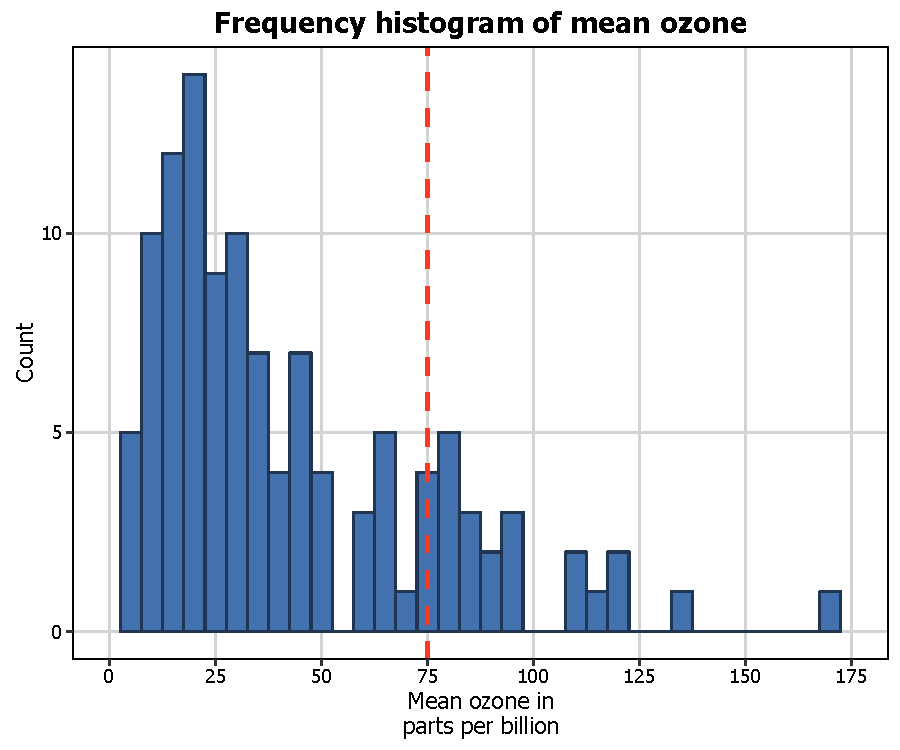
\includegraphics{7_Histograms_pdf/histogram_18-1} \end{center}

\section{Multiple histograms}\label{multiple-histograms}

You can also easily create multiple histograms by the levels of another
variable. There are two options, in separate (panel) plots, or in the
same plot.

\section{In panel plots}\label{in-panel-plots}

We first need to do a little data wrangling. In order to make the graphs
a bit clearer, we've kept only months ``5'' (May) and ``7'' (July) in a
new dataset \texttt{airquality\_trimmed}. We also need to convert this
variable into either a character or factor variable. We have created a
new factor variable \texttt{Month.f}.

In order to produce a panel plot by month, we add the
\texttt{facet\_grid(.\ \textasciitilde{}\ Month.f)} option to the plot.
The additional \texttt{scale\ =\ free} argument in \texttt{facet\_grid}
means that the y-axes of each plot do not need to be the same.

\begin{Shaded}
\begin{Highlighting}[]
\NormalTok{airquality_trimmed <-}\StringTok{ }\NormalTok{airquality[}\KeywordTok{which}\NormalTok{(airquality$Month ==}\StringTok{ }\DecValTok{5} \NormalTok{|}\StringTok{ }
\StringTok{  }\NormalTok{airquality$Month ==}\StringTok{ }\DecValTok{7}\NormalTok{), ]}
\NormalTok{airquality_trimmed$Month.f <-}\StringTok{ }\KeywordTok{factor}\NormalTok{(airquality_trimmed$Month, }
  \DataTypeTok{labels =} \KeywordTok{c}\NormalTok{(}\StringTok{"May"}\NormalTok{, }\StringTok{"July"}\NormalTok{))}

\NormalTok{p7 <-}\StringTok{ }\KeywordTok{ggplot}\NormalTok{(airquality_trimmed, }\KeywordTok{aes}\NormalTok{(}\DataTypeTok{x =} \NormalTok{Ozone)) +}\StringTok{ }
\StringTok{  }\KeywordTok{geom_histogram}\NormalTok{(}\KeywordTok{aes}\NormalTok{(}\DataTypeTok{y =} \NormalTok{..count..), }\DataTypeTok{binwidth =} \DecValTok{10}\NormalTok{,}
    \DataTypeTok{colour =} \NormalTok{barlines, }\DataTypeTok{fill =} \NormalTok{barfill) +}
\StringTok{  }\KeywordTok{scale_x_continuous}\NormalTok{(}\DataTypeTok{name =} \StringTok{"Mean ozone in}\CharTok{\textbackslash{}n}\StringTok{parts per billion"}\NormalTok{,}
    \DataTypeTok{breaks =} \KeywordTok{seq}\NormalTok{(}\DecValTok{0}\NormalTok{, }\DecValTok{175}\NormalTok{, }\DecValTok{25}\NormalTok{), }\DataTypeTok{limits=}\KeywordTok{c}\NormalTok{(}\DecValTok{0}\NormalTok{, }\DecValTok{175}\NormalTok{)) +}
\StringTok{  }\KeywordTok{scale_y_continuous}\NormalTok{(}\DataTypeTok{name =} \StringTok{"Count"}\NormalTok{) +}
\StringTok{  }\KeywordTok{ggtitle}\NormalTok{(}\StringTok{"Frequency histogram of mean ozone"}\NormalTok{) +}
\StringTok{  }\KeywordTok{facet_grid}\NormalTok{(. ~}\StringTok{ }\NormalTok{Month.f, }\DataTypeTok{scales =} \StringTok{"free"}\NormalTok{) +}
\StringTok{  }\KeywordTok{theme}\NormalTok{(}\DataTypeTok{panel.border =} \KeywordTok{element_rect}\NormalTok{(}\DataTypeTok{colour =} \StringTok{"black"}\NormalTok{, }\DataTypeTok{fill=}\OtherTok{NA}\NormalTok{, }\DataTypeTok{size=}\NormalTok{.}\DecValTok{5}\NormalTok{), }
    \DataTypeTok{axis.text.x=}\KeywordTok{element_text}\NormalTok{(}\DataTypeTok{colour=}\StringTok{"black"}\NormalTok{, }\DataTypeTok{size =} \DecValTok{9}\NormalTok{), }
    \DataTypeTok{axis.text.y=}\KeywordTok{element_text}\NormalTok{(}\DataTypeTok{colour=}\StringTok{"black"}\NormalTok{, }\DataTypeTok{size =} \DecValTok{9}\NormalTok{),}
    \DataTypeTok{legend.position=}\StringTok{"bottom"}\NormalTok{, }
    \DataTypeTok{legend.direction=}\StringTok{"horizontal"}\NormalTok{,}
    \DataTypeTok{legend.box =} \StringTok{"horizontal"}\NormalTok{, }
    \DataTypeTok{legend.key.size =} \KeywordTok{unit}\NormalTok{(}\DecValTok{1}\NormalTok{, }\StringTok{"cm"}\NormalTok{),}
    \DataTypeTok{legend.key =} \KeywordTok{element_blank}\NormalTok{(),}
    \DataTypeTok{panel.grid.major =} \KeywordTok{element_line}\NormalTok{(}\DataTypeTok{colour =} \StringTok{"#d3d3d3"}\NormalTok{), }
    \DataTypeTok{panel.grid.minor =} \KeywordTok{element_blank}\NormalTok{(), }
    \DataTypeTok{panel.border =} \KeywordTok{element_blank}\NormalTok{(), }\DataTypeTok{panel.background =} \KeywordTok{element_blank}\NormalTok{(),}
    \DataTypeTok{plot.title =} \KeywordTok{element_text}\NormalTok{(}\DataTypeTok{size =} \DecValTok{14}\NormalTok{, }\DataTypeTok{family =} \StringTok{"Tahoma"}\NormalTok{, }\DataTypeTok{face =} \StringTok{"bold"}\NormalTok{),}
    \DataTypeTok{text=}\KeywordTok{element_text}\NormalTok{(}\DataTypeTok{family=}\StringTok{"Tahoma"}\NormalTok{)) }
\NormalTok{p7}
\end{Highlighting}
\end{Shaded}

\begin{center}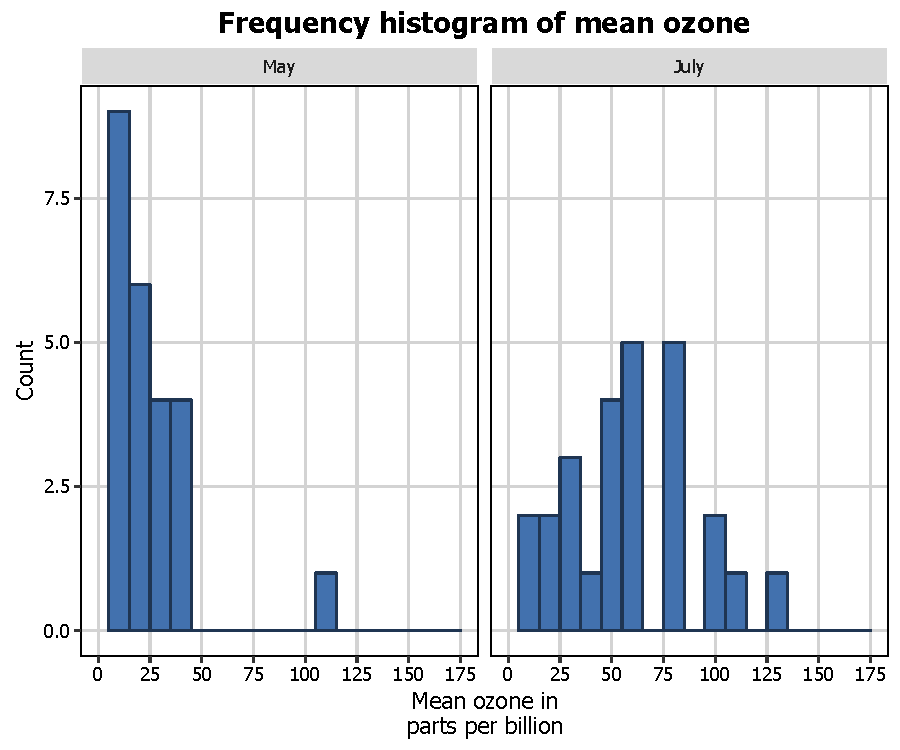
\includegraphics{7_Histograms_pdf/histogram_19-1} \end{center}

\section{In the same plot}\label{in-the-same-plot}

In order to plot the two months in the same plot, we add several things.
Firstly, in the \texttt{ggplot} function, we add a
\texttt{fill\ =\ Month.f} argument to \texttt{aes}. Secondly, in order
to more clearly see the graph, we add two arguments to the
\texttt{geom\_histogram} option, \texttt{position\ =\ "identity"} and
\texttt{alpha\ =\ 0.75}. This controls the position and transparency of
the curves respectively. Finally, you can customise the colours of the
histograms by adding the \texttt{scale\_fill\_brewer} to the plot from
the \texttt{RColorBrewer} package.
\href{http://moderndata.plot.ly/create-colorful-graphs-in-r-with-rcolorbrewer-and-plotly/}{This}
blog post describes the available packages.

\begin{Shaded}
\begin{Highlighting}[]
\NormalTok{p7 <-}\StringTok{ }\KeywordTok{ggplot}\NormalTok{(airquality_trimmed, }\KeywordTok{aes}\NormalTok{(}\DataTypeTok{x =} \NormalTok{Ozone, }\DataTypeTok{fill =} \NormalTok{Month.f)) +}\StringTok{ }
\StringTok{  }\KeywordTok{geom_histogram}\NormalTok{(}\KeywordTok{aes}\NormalTok{(}\DataTypeTok{y =} \NormalTok{..count..), }\DataTypeTok{binwidth =} \DecValTok{10}\NormalTok{,}
    \DataTypeTok{position=}\StringTok{"identity"}\NormalTok{, }\DataTypeTok{alpha=}\FloatTok{0.75}\NormalTok{) +}
\StringTok{  }\KeywordTok{scale_x_continuous}\NormalTok{(}\DataTypeTok{name =} \StringTok{"Mean ozone in}\CharTok{\textbackslash{}n}\StringTok{parts per billion"}\NormalTok{,}
    \DataTypeTok{breaks =} \KeywordTok{seq}\NormalTok{(}\DecValTok{0}\NormalTok{, }\DecValTok{175}\NormalTok{, }\DecValTok{25}\NormalTok{), }\DataTypeTok{limits=}\KeywordTok{c}\NormalTok{(}\DecValTok{0}\NormalTok{, }\DecValTok{175}\NormalTok{)) +}
\StringTok{  }\KeywordTok{scale_y_continuous}\NormalTok{(}\DataTypeTok{name =} \StringTok{"Count"}\NormalTok{) +}
\StringTok{  }\KeywordTok{ggtitle}\NormalTok{(}\StringTok{"Frequency histogram of mean ozone"}\NormalTok{) +}
\StringTok{  }\KeywordTok{scale_fill_brewer}\NormalTok{(}\DataTypeTok{palette=}\StringTok{"Accent"}\NormalTok{) +}
\StringTok{  }\KeywordTok{theme}\NormalTok{(}\DataTypeTok{panel.border =} \KeywordTok{element_rect}\NormalTok{(}\DataTypeTok{colour =} \StringTok{"black"}\NormalTok{, }\DataTypeTok{fill=}\OtherTok{NA}\NormalTok{, }\DataTypeTok{size=}\NormalTok{.}\DecValTok{5}\NormalTok{), }
    \DataTypeTok{axis.text.x=}\KeywordTok{element_text}\NormalTok{(}\DataTypeTok{colour=}\StringTok{"black"}\NormalTok{, }\DataTypeTok{size =} \DecValTok{9}\NormalTok{), }
    \DataTypeTok{axis.text.y=}\KeywordTok{element_text}\NormalTok{(}\DataTypeTok{colour=}\StringTok{"black"}\NormalTok{, }\DataTypeTok{size =} \DecValTok{9}\NormalTok{),}
    \DataTypeTok{legend.position=}\StringTok{"bottom"}\NormalTok{, }
    \DataTypeTok{legend.direction=}\StringTok{"horizontal"}\NormalTok{,}
    \DataTypeTok{legend.box =} \StringTok{"horizontal"}\NormalTok{, }
    \DataTypeTok{legend.key.size =} \KeywordTok{unit}\NormalTok{(}\DecValTok{1}\NormalTok{, }\StringTok{"cm"}\NormalTok{),}
    \DataTypeTok{legend.key =} \KeywordTok{element_blank}\NormalTok{(),}
    \DataTypeTok{panel.grid.major =} \KeywordTok{element_line}\NormalTok{(}\DataTypeTok{colour =} \StringTok{"#d3d3d3"}\NormalTok{), }
    \DataTypeTok{panel.grid.minor =} \KeywordTok{element_blank}\NormalTok{(), }
    \DataTypeTok{panel.border =} \KeywordTok{element_blank}\NormalTok{(), }\DataTypeTok{panel.background =} \KeywordTok{element_blank}\NormalTok{(),}
    \DataTypeTok{plot.title =} \KeywordTok{element_text}\NormalTok{(}\DataTypeTok{size =} \DecValTok{14}\NormalTok{, }\DataTypeTok{family =} \StringTok{"Tahoma"}\NormalTok{, }\DataTypeTok{face =} \StringTok{"bold"}\NormalTok{),}
    \DataTypeTok{text=}\KeywordTok{element_text}\NormalTok{(}\DataTypeTok{family=}\StringTok{"Tahoma"}\NormalTok{)) }
\NormalTok{p7}
\end{Highlighting}
\end{Shaded}

\begin{center}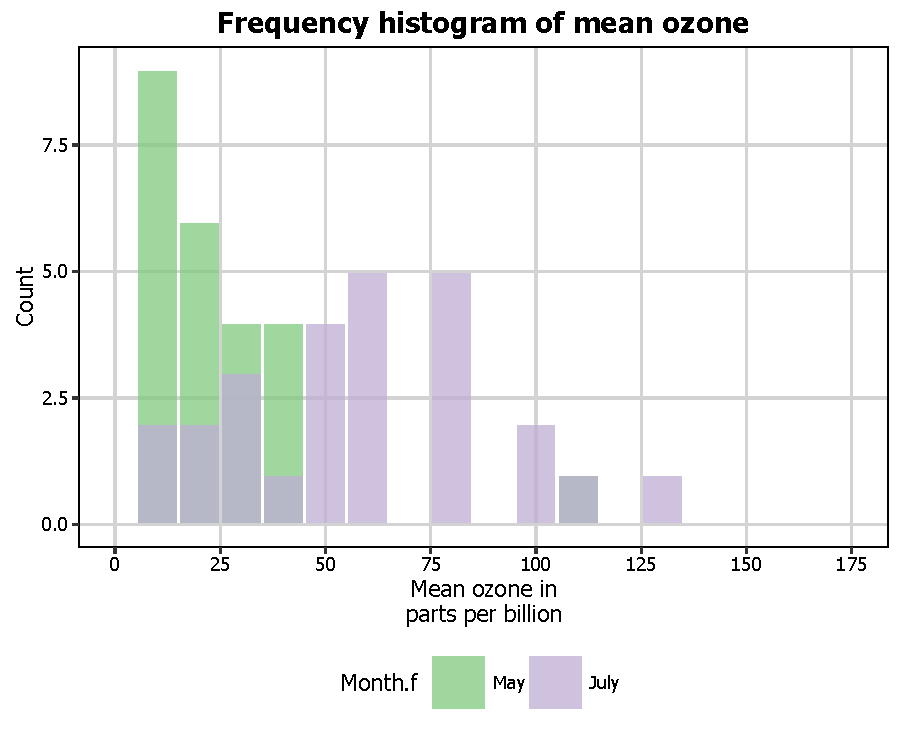
\includegraphics{7_Histograms_pdf/histogram_20-1} \end{center}

\section{Formatting the legend}\label{formatting-the-legend}

Finally, we can format the legend. Firstly, we can change the position
by adding the \texttt{legend.position\ =\ "bottom"} argument to the
\texttt{theme} option, which moves the legend under the plot. Secondly,
we can fix the title by adding the \texttt{labs(fill="Month\ ")} option
to the plot.

\begin{Shaded}
\begin{Highlighting}[]
\NormalTok{p7 <-}\StringTok{ }\KeywordTok{ggplot}\NormalTok{(airquality_trimmed, }\KeywordTok{aes}\NormalTok{(}\DataTypeTok{x =} \NormalTok{Ozone, }\DataTypeTok{fill =} \NormalTok{Month.f)) +}\StringTok{ }
\StringTok{  }\KeywordTok{geom_histogram}\NormalTok{(}\KeywordTok{aes}\NormalTok{(}\DataTypeTok{y =} \NormalTok{..count..), }\DataTypeTok{binwidth =} \DecValTok{10}\NormalTok{,}
    \DataTypeTok{position=}\StringTok{"identity"}\NormalTok{, }\DataTypeTok{alpha=}\FloatTok{0.75}\NormalTok{) +}
\StringTok{  }\KeywordTok{scale_x_continuous}\NormalTok{(}\DataTypeTok{name =} \StringTok{"Mean ozone in}\CharTok{\textbackslash{}n}\StringTok{parts per billion"}\NormalTok{, }
    \DataTypeTok{breaks =} \KeywordTok{seq}\NormalTok{(}\DecValTok{0}\NormalTok{, }\DecValTok{175}\NormalTok{, }\DecValTok{25}\NormalTok{), }\DataTypeTok{limits=}\KeywordTok{c}\NormalTok{(}\DecValTok{0}\NormalTok{, }\DecValTok{175}\NormalTok{)) +}
\StringTok{  }\KeywordTok{scale_y_continuous}\NormalTok{(}\DataTypeTok{name =} \StringTok{"Count"}\NormalTok{) +}
\StringTok{  }\KeywordTok{ggtitle}\NormalTok{(}\StringTok{"Frequency histogram of mean ozone"}\NormalTok{) +}
\StringTok{  }\KeywordTok{scale_fill_brewer}\NormalTok{(}\DataTypeTok{palette=}\StringTok{"Accent"}\NormalTok{) +}
\StringTok{  }\KeywordTok{labs}\NormalTok{(}\DataTypeTok{fill=}\StringTok{"Month "}\NormalTok{) +}
\StringTok{  }\KeywordTok{theme}\NormalTok{(}\DataTypeTok{panel.border =} \KeywordTok{element_rect}\NormalTok{(}\DataTypeTok{colour =} \StringTok{"black"}\NormalTok{, }\DataTypeTok{fill=}\OtherTok{NA}\NormalTok{, }\DataTypeTok{size=}\NormalTok{.}\DecValTok{5}\NormalTok{), }
    \DataTypeTok{axis.text.x=}\KeywordTok{element_text}\NormalTok{(}\DataTypeTok{colour=}\StringTok{"black"}\NormalTok{, }\DataTypeTok{size =} \DecValTok{9}\NormalTok{), }
    \DataTypeTok{axis.text.y=}\KeywordTok{element_text}\NormalTok{(}\DataTypeTok{colour=}\StringTok{"black"}\NormalTok{, }\DataTypeTok{size =} \DecValTok{9}\NormalTok{),}
    \DataTypeTok{legend.position=}\StringTok{"bottom"}\NormalTok{, }
    \DataTypeTok{legend.direction=}\StringTok{"horizontal"}\NormalTok{,}
    \DataTypeTok{legend.box =} \StringTok{"horizontal"}\NormalTok{, }
    \DataTypeTok{legend.key.size =} \KeywordTok{unit}\NormalTok{(}\DecValTok{1}\NormalTok{, }\StringTok{"cm"}\NormalTok{),}
    \DataTypeTok{legend.key =} \KeywordTok{element_blank}\NormalTok{(),}
    \DataTypeTok{panel.grid.major =} \KeywordTok{element_line}\NormalTok{(}\DataTypeTok{colour =} \StringTok{"#d3d3d3"}\NormalTok{), }
    \DataTypeTok{panel.grid.minor =} \KeywordTok{element_blank}\NormalTok{(), }
    \DataTypeTok{panel.border =} \KeywordTok{element_blank}\NormalTok{(), }\DataTypeTok{panel.background =} \KeywordTok{element_blank}\NormalTok{(),}
    \DataTypeTok{plot.title =} \KeywordTok{element_text}\NormalTok{(}\DataTypeTok{size =} \DecValTok{14}\NormalTok{, }\DataTypeTok{family =} \StringTok{"Tahoma"}\NormalTok{, }\DataTypeTok{face =} \StringTok{"bold"}\NormalTok{),}
    \DataTypeTok{text=}\KeywordTok{element_text}\NormalTok{(}\DataTypeTok{family=}\StringTok{"Tahoma"}\NormalTok{)) }
\NormalTok{p7}
\end{Highlighting}
\end{Shaded}

\begin{center}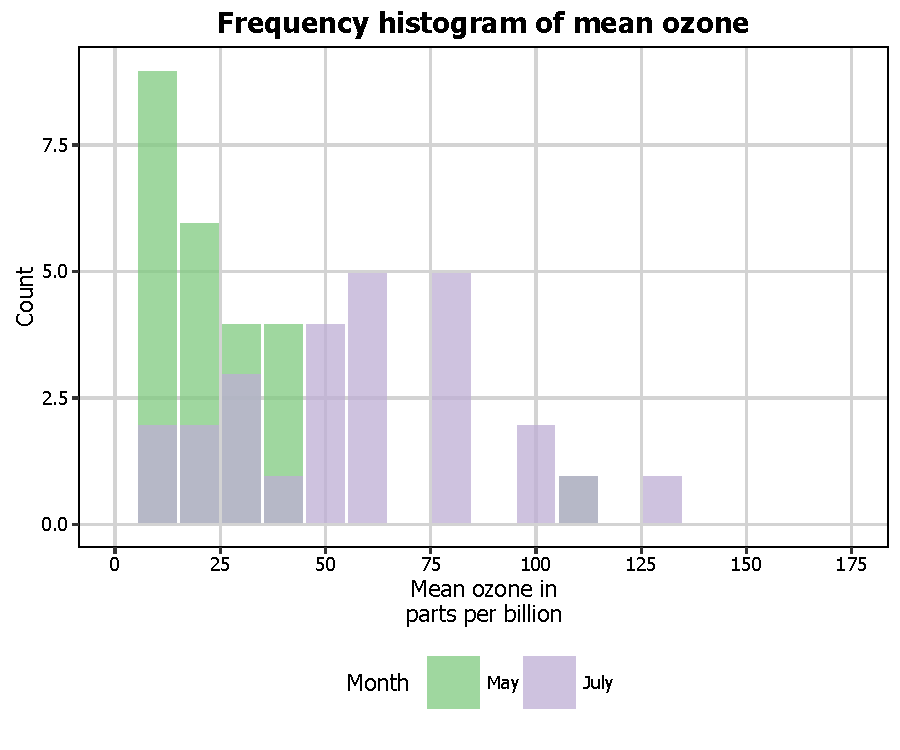
\includegraphics{7_Histograms_pdf/histogram_21-1} \end{center}

\end{document}
